\documentclass[article,shortnames,nofooter]{jss}

%%%%%%%%%%%%%%%%%%%%%%%%%%%%
%% Packages
%%%%%%%%%%%%%%%%%%%%%%%%%%%%
\usepackage{amsmath, amssymb}
\usepackage{bm}
\usepackage{graphicx}
\usepackage{subcaption}
\usepackage{booktabs}
\usepackage{float}
\usepackage{tikz}
\usepackage{multirow}
\usepackage{hhline}
\usepackage[font=small]{caption}
\usetikzlibrary{positioning}
\usetikzlibrary{arrows.meta}

%%%%%%%%%%%%%%%%%%%%%%%%%%%%
%% Title & Authors
%%%%%%%%%%%%%%%%%%%%%%%%%%%%
\title{\pkg{capnet}: Contribution-Capped Regularization for Elastic Net Models in R}

\author{
  %%Harry He\\UC San Diego
}

\Plainauthor{Harry He}
\Plaintitle{\pkg{capnet}: Contribution-Capped Regularization for Elastic Net Models in R}
\Shorttitle{\pkg{capnet}: Contribution-Capped Regularization}

\Abstract{
    \pkg{capnet} is an \proglang{R} package that extends elastic net regression by introducing a contribution-capped regularization framework for controlling predictor influence and improving stability in generalized linear models. Motivated by tactical asset allocation problems where single feature dominance can lead to undesirable concentration risk, \pkg{capnet} allows users to specify feature-specific contribution ceilings and achieves more stable predictions especially in the presence of heavy-tailed predictors. Similar applications arise in risk management, credit scoring, and epidemiology, where extreme covariate realizations can induce large predictor contributions. This paper presents the statistical formulation of contribution caps, their integration with GLMs, and the optimization algorithm used for estimation. We demonstrate the utility of \pkg{capnet} through simulation studies and real-world case studies in finance and risk modeling, showing that contribution-capped models can outperform classical approaches and alternative methods.

    \pkg{capnet} is an \proglang{R} package for fitting generalized linear models with explicit control over predictor influence. In many applications, extreme covariate values can cause a small number of predictors to dominate predictions, leading to instability and concentration risk even in well-regularized models. \pkg{capnet} extends elastic net regression by limiting the contribution of each predictor, improving stability while preserving predictive signal. The framework applies broadly across model families and supports flexible evaluation settings, including stress scenarios and out-of-sample environments. Simulation and empirical applications show that \pkg{capnet} yields more stable and often better predictions, particularly in settings with heavy-tailed predictors or rare but influential observations.
}

\Keywords{regularization, constrained optimization, elastic net, R}
\Plainkeywords{regularization, constrained optimization, elastic net, R}

%%%%%%%%%%%%%%%%%%%%%%%%%%%%
%% Start Document
%%%%%%%%%%%%%%%%%%%%%%%%%%%%
\begin{document}

\section{Introduction}

In many predictive applications, model behavior is driven by how much individual features contribute to the final prediction. When covariates take extreme values, a small number of predictors can dominate the model output, leading to unstable predictions, excessive sensitivity to rare events, or violations of domain-specific constraints. This issue is particularly pronounced in settings with heavy-tailed predictors or when models are evaluated under stress scenarios or out-of-sample conditions, where extreme realizations play a central role. Classical penalization methods such as ridge regression \citep{hoerl1970}, the lasso \citep{tibshirani1996}, and the elastic net \citep{zou2005} control model complexity by shrinking coefficients, but are agnostic to the realized contributions of predictors. Robust regression techniques and alternative distributions or transformations address instability arising from extreme observations or residuals in different ways, but do not provide explicit control over how individual predictors contribute to model outputs.

This issue is particularly salient in quantitative finance applications, where predictors often exhibit heavy-tailed behavior and extreme realizations are central to model evaluation. In such settings, a small number of predictors can induce large swings in fitted values, leading to concentration risk and unstable downstream decisions. Similar challenges arise in risk management, credit scoring, epidemiology, and related fields, where predictors may display skewed or heavy-tailed distributions and predictions are evaluated under stress scenarios rather than average conditions.

This paper introduces \pkg{capnet}, a penalized regression framework and accompanying \proglang{R} package that directly constrains predictor contributions. \pkg{capnet} extends the elastic net by placing feature-specific limits on how much each predictor can influence the linear predictor, providing a direct mechanism for controlling instability and concentration of predictive weight. A key feature of the framework is the ability to specify an evaluation matrix distinct from the training data, allowing contribution constraints to be enforced not only in-sample but also in stress scenarios or anticipated deployment environments. This formulation integrates naturally with generalized linear models and can be efficiently estimated using standard optimization techniques.

The contribution-cap formulation integrates naturally with generalized linear models and yields a convex optimization problem that can be efficiently solved using quasi-Newton methods. The \pkg{capnet} package provides a practical and extensible implementation, including functionality for model fitting, cross-validation, and sequential (walk-forward) estimation, with an interface designed to align with established tools for penalized regression.

The primary contribution of this work is both conceptual and computational. \pkg{capnet} introduces a new dimension of regularization by shifting the focus from controlling parameter magnitude to controlling feature-level influence. By embedding contribution control directly into the estimation procedure, the framework aligns statistical modeling with practical constraints on predictor behavior in applications where stability, robustness, and interpretability are of central importance.

The remainder of this article is organized as follows. Section~\ref{sec:motivate} discusses the practical motivations underlying contribution caps and reviews related approaches for handling heavy-tailed predictors. Section~\ref{sec:framework} presents the contribution-cap framework and its integration with generalized linear models. Section~\ref{sec:software} describes the software implementation and optimization strategy used in the \pkg{capnet} package. Section~\ref{sec:examples} provides empirical examples illustrating the use of \pkg{capnet} in Gaussian and GLM settings. Section~\ref{sec:conclusion} concludes with a discussion of limitations and directions for future research.

\section{Motivations}\label{sec:motivate}

\subsection{Theoretical Motivations}
Contribution caps are motivated by predictive settings in which a small number of predictors can exert disproportionate influence on fitted values, particularly in regions of the covariate space that are rare but substantively important. Consider a predictive task governed by the data generating process shown in Figure~1, where predictors $X_1, \ldots, X_p$ jointly determine the response $Y$.


In an idealized setting, where $X \in \mathbb{R}^{n \times p}$ is fully observed, $n \gg p$, the functional form is linear and additive, and classical assumptions hold, ordinary least squares yields the best linear unbiased estimator (BLUE), and no penalization is required. In practice, deviations from this setting—such as multicollinearity, high-dimensionality, or model misspecification—motivate the use of $\ell_1$ and $\ell_2$ regularization to stabilize estimation.

% \begin{figure}[H]
%     \centering
%     \begin{tikzpicture}[
%         node distance=1.5cm and 1.2cm,
%         every node/.style={draw, circle, minimum size=8mm}
%     ]

%         % X nodes (you can change p as needed)
%         \node (x1) {$X_1$};
%         \node (x2) [right=of x1] {$X_2$};
%         \node (x3) [right=of x2] {$X_3$};
%         \node (xdots) [right=of x3, draw=none] {$\cdots$};
%         \node (xp) [right=of xdots] {$X_p$};

%         % Y node
%         \node (y) [below=1.8cm of x3] {$Y$};

%         % Edges from all X's to Y
%         \draw[-{Latex[length=2mm]}, shorten >=2pt] (x1) -- (y);
%         \draw[-{Latex[length=2mm]}, shorten >=2pt] (x2) -- (y);
%         \draw[-{Latex[length=2mm]}, shorten >=2pt] (x3) -- (y);
%         \draw[-{Latex[length=2mm]}, shorten >=2pt] (xp) -- (y);

%     \end{tikzpicture}
%     \caption{Directed Acyclic Graph for Data Generating Process}
%     \label{fig:dag}
% \end{figure}

The setting motivating contribution caps is different. In many applications, predictors exhibit heavy-tailed or highly heterogeneous behavior, and predictive performance is not evaluated uniformly across the covariate space but instead within specific regions of interest. These regions may constitute only a small fraction of the training data yet dominate the practical objective---for example, periods of market stress in finance, extreme environmental conditions in climate modeling, or rare risk profiles in insurance and credit scoring. In such settings, extreme covariate realizations can induce large realized contributions $X_{ij}\beta_j$, even when coefficients are heavily regularized. This creates a form of instability that is not captured by traditional regularization: a model may appear well-behaved in-sample, yet produce predictions dominated by a small number of predictors when evaluated in these regions. The root cause is that classical methods control coefficient magnitude rather than the realized influence of predictors.

A substantial literature on fat-tailed data addresses related issues indirectly by focusing on heavy-tailed response variables rather than heavy-tailed predictors. Common approaches include transforming the response, adopting generalized linear models with heavy-tailed distributions (e.g., Gamma or inverse Gaussian), using generalized distribution regressions, quantile regression, mixture models, or spliced distributions \citep{shi2014, gan2018}. These methods improve modeling of the conditional distribution of $Y$ but leave the mapping from predictors to the linear predictor unchanged. As a result, they do not regulate predictor contributions and do not prevent extreme covariate realizations from dominating fitted values.

\subsection{Related Approaches}

Practitioners have proposed a variety of strategies to mitigate the effects of heavy-tailed predictors in regression models. These approaches include preprocessing techniques such as transformations and winsorization, robust regression and leverage-based methods, and post-hoc modifications to fitted values. While each of these methods addresses certain aspects of instability induced by extreme covariate realizations, they do so indirectly and do not provide explicit control over the realized contributions of predictors to the linear predictor.

Preprocessing techniques such as logarithmic, power, or rank-based transformations, as well as winsorization and trimming, are commly used to compress the tail of predictor distributions prior to model fitting. These methods can reduce the influence of extreme observations and improve numeric stability. However, they operate independently of the fitted model, require heuristic choices of transformation or truncation thresholds, and alter the scale and interpretation of predictors. Moreover, they provide no guarantees against extreme predictor realizations encountered in new or stress scenarios. 

Robust regression techniques, including M-estimators, reduce the influence of extreme observations by downweighting points with large residuals or high leverage, thereby stabilizing coefficient estimation under heavy-tailed noise \citep{huber1973}. Relatedly, distributionally robust optimization (DRO) methods introduce robustness by minimizing worst-case expected loss over a neighborhood of plausible data-generating distributions \citep{bental2009}. In both cases, robustness is achieved through modifications to the loss or weighting scheme and operates primarily at the level of residuals or aggregate predictive risk. However, neither framework directly regulates the realized contributions of individual predictors to the linear predictor, and high-leverage covariate realizations with small residuals may still exert disproportionate influence. Consequently, even models estimated using robust regression or DRO can produce large predictor contributions in new or stress scenarios, as these methods do not impose explicit bounds on $X_{ij}\beta_j$.

Another common strategy is to impose constraints on the linear predictor or fitted values after model estimation. While such post-hoc approach can prevent extreme predictions, they disconnect the estimation procedure from the constraints applied at deployment, as the model is not estimated under the same restrictions that govern its use. This mismatch can lead to suboptimal coefficient estimates and reduced predictive performance. 

In addition to these methdological approaches, several software packages provide penalized or constrained generalized linear model fitting. The \pkg{glmnet} package \citep{friedman2010} implements efficient algorithms for $\ell_1$- and $\ell_2$-regularized GLMs, but regularization acts only on the coefficient vector and does not constrain realized predictor contributions. Packages such as \pkg{mgcv} \citep{wood2017} impose smoothness or shape constraints on functional relationships, while bias-reduction methods such as \pkg{brglm2} \citep{kosmidis2019} address small-sample bias and separation issues. Although these tools provide valuable forms of regularization and stabilization, they do not offer mechanisms for directly bounding the influence of individual predictors.

Taken together, existing approaches can be understood as targeting different components of model instability: preprocessing methods modify the distribution of predictors, robust regression methods control the influence of observations through residuals, and DRO methods address uncertainty in the data-generating process. However, none of these approaches directly constrain predictor-level contributions, leaving open the possibility that a small number of predictors may dominate model outputs when covariates take extreme values.

Contribution caps address this gap by integrating influence constraints directly into the estimation problem. Rather than modifying predictors ex ante or predictions ex post, the cap penalty operates on realized contributions $Z_{ij}\beta_j$ during optimization. This ensures that predictor influence is bounded in the regions of the covariate space encoded by the evaluation matrix $Z$, while preserving the probabilistic structure of the underlying GLM. By allowing $Z$ to differ from the training design matrix, contribution caps provide a principled mechanism for enforcing stability not only on observed data but also on stress scenarios or anticipated deployment environments. Importantly, this approach does not rely on fitting separate models across regimes. Instead, \pkg{capnet} incorporates regime-specific considerations within a single estimation problem by enforcing contribution constraints over the evaluation matrix $Z$. The resulting model adapts its effective behavior across different regions of the covariate space through the optimization objective, while maintaining a unified and interpretable parameterization.

\subsection{Motivating Example}

In this subsection, we present two simplified linear regression examples that illustrate the theoretical considerations discussed above and demonstrate practical use cases for \pkg{capnet}.

First, we consider a simulated setting in which the outcome variable $y$ is generated from a latent feature matrix $Z$ according to a linear data generating process. In estimation and prediction, however, the analyst does not observe $Z$ directly but instead observes a noisy proxy matrix $X$, whose distribution exhibits heavier tails for a subset of predictors. This setup can be interpreted as a measurement error problem in which the observed covariates are imperfect and heteroskedastic proxies for the true latent features.

Formally, the outcome is generated as
\[
y_i = Z_i \beta + \varepsilon_i, \quad \varepsilon_i \sim \mathcal{N}(0, \sigma^2),
\]
where $\beta$ is a sparse coefficient vector.\footnote{Sparsity is introduced by randomly setting a subset of coefficients to zero.}

The observed covariates are constructed by adding noise to $Z$. Features are partitioned into a stable set $\mathcal{S}$ and an unstable set $\mathcal{U}$. For features in $\mathcal{S}$, the added noise is homoskedastic Gaussian:
\[
\eta_{ij} \sim \mathcal{N}(0, \sigma_{\text{low}}^2), \quad j \in \mathcal{S}.
\]
For features in $\mathcal{U}$, the noise variance varies across observations, mimicking leptokurtic measurement error. Specifically, for each observation $i$ and feature $j \in \mathcal{U}$, we draw
\[
F_{ij} \sim \text{Bernoulli}(p),
\]
and define
\[
s_{ij} =
\begin{cases}
\sigma_{\text{low}}, & F_{ij} = 0, \\
\sigma_{\text{high}}, & F_{ij} = 1.
\end{cases}
\]
Conditional on $F_{ij}$, the noise term follows
\[
\eta_{ij} \mid F_{ij} \sim \mathcal{N}(0, s_{ij}^2).
\]
The observed design matrix is then given by $X = Z + \eta$.

This data generating process produces covariates that are heteroskedastic and heavy-tailed for unstable features. When estimating linear models using $X$, conventional methods may encounter two related challenges. First, extreme realizations can exert disproportionate influence on coefficient estimates, leading to instability and degraded out-of-sample performance. Second, large covariate realizations may induce excessive concentration of predictive weight in a small number of features, allowing individual predictors to dominate the magnitude and direction of predictions. Importantly, the second issue persists even when coefficient shrinkage is applied. Because classical regularization methods act on $\beta$ rather than on realized contributions $X_{ij}\beta_j$, extreme covariate realizations can still generate large contributions and dominate model outputs.

In settings where Gaussian assumptions for covariates are appropriate, such extreme observations may be treated as outliers and addressed using winsorization or robust loss functions. However, when the covariate distribution is genuinely heavy-tailed or when it is difficult to distinguish informative extreme values from noise, these approaches may systematically downweight predictive features and degrade performance. By contrast, \pkg{capnet} allows features to retain predictive influence while explicitly limiting their contribution to the fitted values, enabling control over feature dominance without discarding extreme observations.

To evaluate performance, the data are split into training and testing sets. The elastic net tuning parameter $\lambda$ is selected via cross-validation with an equal mixture of $\ell_1$ and $\ell_2$ penalties. For \pkg{capnet}, we consider multiple configurations: (i) global evaluation on the full test matrix versus walk-forward evaluation in which models are refit sequentially, (ii) a range of penalty strengths, and (iii) varying contribution ceiling levels.\footnote{Contribution ceilings are computed as multiples of the univariate regression coefficients between each feature and the outcome in the training set.}

Each configuration is compared against the unconstrained elastic net benchmark, corresponding to a zero contribution cap. Tables~\ref{tab:simulate_full} and~\ref{tab:simulate_walk} report out-of-sample performance for the full and walk-forward evaluation schemes, respectively.

\begin{table}[H]
    \centering
    \begin{tabular}{|cc|ccccc|}
        \hhline{|=======|}
        & & \multicolumn{5}{|c|}{Contribution Ceiling Multiplier} \\
        & & $0$ & $2$ & $4$ & $8$ & $16$\\
        \hline
        \multirow{5}{*}{Penalty Strength} & $0$ & $8.650$ & & & &\\
        & $0.1$ & & $8.536$ & $8.441$ & $8.571$ & $8.650$\\
        & $1$ & & $9.071$ & $8.353$ & $8.527$ & $8.650$\\
        & $10$ & & $9.650$ & $8.341$ & $8.519$ & $8.650$\\
        & $100$ & & $9.762$ & $8.340$ & $8.519$ & $8.650$\\
        \hhline{|=======|}
    \end{tabular}
    \caption{Out-of-sample mean squared error (MSE) for capnet models on the simulated dataset. The case $\gamma=0$ and $\text{multiplier} = 0$ corresponds to the uncapped elastic net benchmark. Moderate contribution ceilings (e.g., multipliers of 2–4) improve predictive performance relative to the uncapped model.}
    \label{tab:simulate_full}
\end{table}

\begin{table}[H]
    \centering
    \begin{tabular}{|cc|ccccc|}
        \hhline{|=======|}
        & & \multicolumn{5}{|c|}{Contribution Ceiling Multiplier} \\
        & & $0$ & $2$ & $4$ & $8$ & $16$\\
        \hline
        \multirow{5}{*}{Penalty Strength} & $0$ & $8.650$ & & & &\\
        & $0.1$ & & $8.098$ & $8.104$ & $8.412$ & $8.650$\\
        & $1$ & & $8.118$ & $8.096$ & $8.405$ & $8.650$\\
        & $10$ & & $8.124$ & $8.095$ & $8.404$ & $8.650$\\
        & $100$ & & $8.124$ & $8.095$ & $8.404$ & $8.650$\\
        \hhline{|=======|}
    \end{tabular}
    \caption{Out-of-sample mean squared error (MSE) of walk-forward \pkg{capnet} models on the simulated dataset. Each model is refit sequentially along the evaluation path. All capped specifications outperform the uncapped benchmark, illustrating that local contribution control improves predictive stability and accuracy relative to global constraints.}
    \label{tab:simulate_walk}
\end{table}

Across configurations, \pkg{capnet} frequently outperforms the benchmark model, although excessively restrictive ceilings can degrade performance. Conversely, when ceilings are sufficiently large, the constraint becomes inactive and the solution reduces to the unconstrained elastic net. While the penalty strength affects performance, particularly when contribution ceilings are tight, its influence is generally smaller than that of the ceiling level itself, highlighting the importance of selecting appropriate contribution limits. The walk-forward evaluation approach consistently delivers improved performance and greater stability. This behavior reflects the fact that imposing global contribution constraints over an entire evaluation set can lead to overly aggressive penalization, whereas local, observation-level constraints adapt more flexibly to changing covariate realizations. As discussed further in the software implementation section, the walk-forward approach is generally preferred despite its higher computational cost, particularly when heuristics for selecting contribution ceilings are imperfect.

Second, consider an application in quantitative finance. In a medium-frequency market-timing model, a set of predictors is used to forecast excess equity risk premia. Financial predictors are often noisy and heavy-tailed, making it difficult to distinguish meaningful extreme values from noise. A central challenge is to construct a model that captures informative deviations from long-run patterns while maintaining a well-controlled risk profile. This includes limiting the extent to which any single feature can influence model predictions, as highly dominant predictors can create concentration risk and lead to unstable portfolio outcomes. In such settings, contribution caps provide a direct mechanism for controlling feature-level influence while preserving predictive signal. More details will be discussed in Section~\ref{sec:examples}.

\section{The Contribution-Cap Framework}\label{sec:framework}

\subsection{Model Setup}

Let $y \in \mathbb{R}^n$ denote the response vector and $X \in \mathbb{R}^{n \times p}$ the predictor matrix, with rows $X_i^\top$ representing observations and columns $X_{\cdot j}$ representing predictors. Consider a generalized linear model with canonical link, under which the linear predictor is
\[
\eta = X\beta,
\]
The \pkg{capnet} package supports model families for which the negative log-likelihood is smooth and convex in $\eta$, ensuring that the resulting penalized estimation problem remains convex.

For Gaussian regression with identity link, the negative log-likelihood is
\[
\ell(y,\beta, X) = \frac{1}{2}\|y - X\beta\|_2^2.
\]
For logistic regression (binomial with logit link),
\[
\ell(y,\beta,X) = \sum_{i=1}^n \left[ \log\!\left(1 + e^{x_i\beta}\right) - y_ix_i\beta \right].
\]
For Poisson regression with log link,
\[
\ell(\beta) = \sum_{i=1}^n \left( e^{x_i\beta} - y_i x_i\beta \right).
\]
For Gamma regression with log link and fixed shape parameter,
\[
\ell(\beta) = \sum_{i=1}^n \left( y_i e^{-x_i\beta} + x_i\beta \right).
\]

These families cover the most commonly used GLMs in applied work and share a convenient structure: the likelihood depends on $\beta$ only through the linear predictor $X\beta$ and yields a convex optimization landscape. This property allows \pkg{capnet} to incorporate additional penalties without altering the fundamental estimation framework.

\subsection{Contribution Caps}

A distinctive feature of \pkg{capnet} is that contribution caps are computed not necessarily on the training matrix $X$, but on a user-supplied evaluation matrix $Z \in \mathbb{R}^{m \times p}$. Each row of $Z$ represents an evaluation scenario, and each column corresponds to a predictor. This flexibility allows users to regulate predictor influence not only on the training data but also on future or representative environments---an important consideration in applications such as forecasting, risk modeling, or market-timing systems where large contributions may manifest primarily in out-of-sample conditions.

For observation $i$ and predictor $j$, the realized contribution of predictor $j$ in evaluation context $Z$ is
\[
Z_{ij}\beta_j.
\]
\pkg{capnet} imposes a soft upper bound on these realized contributions via
\[
|Z_{ij}\beta_j| \le L_j,
\]
where $L_j > 0$ is a user-specified cap. Violations of this constraint are penalized through the smooth hinge-squared penalty
\[
C(\beta,Z,L)
=
\sum_{j=1}^p\sum_{i=1}^m \left( |Z_{ij}\beta_j| - L_j \right)_+^2,
\qquad
(z)_+ = \max(z,0).
\]

This penalty activates only when the magnitude of a predictor’s contribution exceeds its cap and then grows quadratically. Because the hinge-squared function is continuously differentiable, it is directly compatible with gradient-based optimization methods.

The interpretation of $L_j$ is unified across GLM families because all models operate through the linear predictor. In Gaussian models, $Z_{ij}\beta_j$ is an additive contribution to the estimated mean; bounding it directly limits additive influence. In logistic regression, $Z_{ij}\beta_j$ is a change in log-odds, so the cap limits the corresponding odds multiplier to lie within $[e^{-L_j}, e^{L_j}]$. In Poisson and Gamma regression, $Z_{ij}\beta_j$ adjusts the log-mean, yielding a multiplicative bound on the expected count or positive-valued outcome. A single formulation therefore provides additive control in Gaussian models and multiplicative control in log- and logit-link GLMs.

\subsection{Penalized Estimation}

The \pkg{capnet} estimator solves the convex optimization problem
\begin{equation}
\hat\beta
=
\arg\min_{\beta \in \mathbb{R}^p}
\left\{
    \ell(y,\beta,X)
    +
    \lambda\!\left[\frac{1-\alpha}{2}\|\beta\|_2^2 + \alpha\|\beta\|_1\right]
    +
    \gamma\, C(\beta,Z,L)
\right\}
\label{eq:loss}
\end{equation}
where $\lambda \ge 0$ controls the overall intensity of coefficient regularization, $\alpha \in [0,1]$ determines the balance between $\ell_1$ and $\ell_2$ penalties, and $\gamma \ge 0$ controls the strength of the contribution-cap penalty. This formulation mirrors the elastic-net parameterization familiar from \citet{friedman2010} and allows users to employ ridge-like, lasso-like, or hybrid regularization alongside contribution caps.

A key design feature is the explicit separation of the training matrix $X$ and the evaluation matrix $Z$. When $Z = X$, \pkg{capnet} regulates contributions on the training data, recovering the standard setting. When $Z$ differs from $X$---such as when $Z$ contains representative future market states, stress scenarios, or held-out data---\pkg{capnet} ensures that predictor influence remains bounded even in environments that may not be presented in the training sample. This provides a principled mechanism for controlling contribution‐level instability or concentration risk in downstream predictive tasks.

The three penalty components interact in complementary ways. The $\ell_1$ term enables sparsity, the $\ell_2$ term improves numerical stability in the presence of multicollinearity, and the contribution-cap penalty regulates large or volatile contributions. Setting $\gamma=0$ recovers classical penalized GLMs; setting $\lambda=0$ yields a pure contribution-regularized model; and using both penalties allows simultaneous control of coefficient magnitude and predictor influence.

Because the hinge-squared cap penalty is convex and smooth, and the GLM likelihoods considered are convex in the linear predictor, the overall objective remains convex and continuously differentiable except for the nondifferentiability introduced by the $\ell_1$ term. This structure is well suited to limited-memory quasi-Newton optimization and provides stable convergence across model families and evaluation matrices.

\subsection{Optimization}

As discussed above, the negative likelihood function (\ref{eq:loss}) is smooth and convex for all supported GLM families. The only source of nondifferentiability arises from the $\ell_1$ term. These properties make the objective well suited to limited-memory quasi-Newton methods. \pkg{capnet} uses the \pkg{lbfgs} package for optimization \cite{lbfgs}. When $\alpha=0$, the objective function is fully smooth, and standard L-BFGS method is applied. When $\alpha>0$, the $\ell_1$ component introduces non-smoothness at zero, and the optimizer automatically switches to the orthant-wise limited-memory quasi-Newton (OWL-QN) method, which handles the $\ell_1$ subgradient by restricting updates to remain within the current orthant, enabling quasi-Newton updates while preserving sparsity-inducing behavior \cite{andrew2007}.

Calling the \pkg{lbfgs} optimizer requires the objective and gradient functions. From (\ref{eq:loss}), we calculate the gradient as
\begin{equation}
    \nabla \mathcal{L}(\beta)=\nabla \ell(y,\beta,X)
+
\lambda\Big[(1-\alpha)\beta + \alpha\,\partial\|\beta\|_1\Big]
+
\gamma\, \nabla C(\beta,Z,L)
\label{eq:gradient}
\end{equation}

The first component is the standard GLM score
\[\nabla \ell(y,\beta,X)=X^\top(\mu - y),\qquad\mu = g^{-1}(X\beta)\]
And for the contribution-cap penalty, the gradient is
\[
\frac{\partial C}{\partial \beta_j}
=
2\sum_{i=1}^m\left(|Z_{ij}\beta_j| - L_j\right)_+
\cdot
\mathrm{sign}(Z_{ij}\beta_j)
Z_{ij}.
\]
The hinge-squared form ensures differentiability even at the activation boundary.

Also define the contribution matrix as 
\[A=Z\text{ diag}(\beta)\in\mathbb R^{m\times p}\]
$S=\text{sign}(A)$ element-wise, and $V=(|A|-\bm{1}L^\top)_+$. The gradient of the contribution-cap penalty can be written in the following matrix form:
\[\nabla_\beta C=2\Big((V\odot S)\odot Z\Big)^\top\bm{1}\in\mathbb R^p\]
where $\odot$ is element-wise multiplication, and this is how the gradient calculation is performed in the \pkg{capnet} package.

The evaluation matrix $Z$ enters the optimization only through the penalty term. Because $C(\beta,Z,L)$ decomposes additively over predictors, the cost of computing its gradient grows linearly in the number of rows of $Z$. This design allows users to specify large or diverse evaluation sets without affecting the GLM likelihood computation.

\section{Software Implementation and Example Usage}\label{sec:software}

\begin{table}[h]
    \centering
    \begin{tabular}{lp{9cm}}
    \hline\hline
        Function & Purpose \\
    \hline \\[-0.3cm]
        \code{simulate_capnet_data()} & Generates simulated data for linear regression experiments and examples. \\[0.6em]
        \code{capnet()} & Fits a contribution-capped elastic net regression model for a fixed set of hyper-parameters. \\[0.6em]
        \code{walk_capnet()} & Computes a sequence of \code{capnet} models along a user-specified path of the evaluation dataset. \\[0.6em]
        \code{cv_capnet()} & Performs cross-validation over a grid of elastic net hyper-parameters to select a preferred model specification. \\[0.6em]
        \code{coef_path()} & Extracts regression coefficients from a collection of fitted \code{capnet} models along a hyper-parameter path. \\[0.6em]
        \code{capnet_violations()} & Identifies and summarizes violations of the soft contribution-cap constraints for a fitted \code{capnet} model. \\[0.6em]
        \code{plot_redistribution()} & Visualizes changes in regression coefficients and feature-level contributions between two fitted \code{capnet} models. \\[0.1cm]
    \hline\hline
    \end{tabular}
    \caption{Primary user-facing functions provided by the \pkg{capnet} package.}
    \label{tab:capnet-functions}
\end{table}

This section provides a simple illustration of using the \pkg{capnet} package to fit the contribution-capped elastic net regression models. We will mostly consider the linear regression model and then briefly discuss extensions to the logistic, Poisson, and gamma regression cases. The package is available from ... and can be installed and loaded in the usual manner:

\begin{Code}
    R> install.packages("capnet")
    R> library("capnet")
\end{Code}

We first load a small simulated dataset, including the training design matrix and response vector, the contribution cap vector, and evaluation design matrix, using the built-in \\\code{simulate_capnet_data()} function.

\begin{Code}
    R> n <- 100
    R> p <- 10
    R> m <- 20
    R> data <- simulate_capnet_data(n=100,p=10,m=20)
    R> X <- data$X
    R> y <- data$y
    R> L <- data$L
    R> newx <- data1$newx
\end{Code}

The \pkg{capnet} package is mainly used with calls to estimation three functions as shown in Table~\ref{tab:capnet-functions}: \code{capnet()}, \code{walk_capnet()}, and \code{cv_capnet()}. The interface is designed to mimic popular \proglang{R} packages for regularized generalized linear models, most notably \pkg{glmnet} \citep{friedman2010}. To perform the contribution-capped regression, \code{capnet()} takes as required inputs, the design matrix \code{x}, the response vector \code{y}, and the contribution cap vector \code{L}. The function also take several optional arguments. The \code{newx} matrix specifies the evaluation matrix for the feature contributions. The \code{family} argument specifies the regression model (\code{"gaussian"}, \code{"binomial"}, \code{"poisson"}, or \code{"gamma"}). \code{alpha}, \code{lambda}, and \code{gamma} controls the elastic net and contribution cap penalty strengths, and \code{upper.limits} and \code{lower.limits} vectors specify coefficients box constraints. 

By default, the model fits a Gaussian model using the training design matrix \code{X} as the evaluation matrix and adds no elastic net or contribution cap penalties and no box constraints. Below are sample usages with different combinations of parameters

\begin{Code}
    # No regularization, same as running lm()
    R> fit1 <- capnet(X, y, L)
    
    # Only elastic net penalties, same as running glmnet()
    R> alpha <- 0.5
    R> lambda <- 0.1
    R> fit2 <- capnet(X, y, L, alpha = alpha, lambda = lambda)
    
    # Adding contribution cap penalties, evaluated on training design matrix
    R> gamma <- 1
    R> fit3 <- capnet(X, y, L, alpha = alpha, lambda = lambda, gamma = gamma)
    
    # Evaluating capnet on evaluation matrix
    R> fit4 <- capnet(X, y, L, newx = newx, alpha = alpha, lambda = lambda, 
    +    gamma = gamma)
    
    # Adding box constraints
    upper.limits <- c(rep(Inf, 5), rep(0, 5))
    lower.limits <- c(rep(0, 5), rep(-Inf, 5))
    R> fit5 <- capnet(X, y, L, newx = newx, alpha = alpha, lambda = lambda, 
    +    gamma = gamma, lower.limits = lower.limits, upper.limits = upper.limits)
\end{Code}

\code{capnet()} returns an \code{S3} object, and we have included the \code{coef} and \code{predict} functions to display the coefficients and make predictions on new design matrix data.

\begin{CodeChunk}
\begin{CodeInput}
    R> coef(fit4)
\end{CodeInput}
\begin{CodeOutput}
                       beta
    (Intercept) -0.04415975
    X1           0.51001177
    X2          -1.71345010
    X3           1.02256470
    X4          -1.02555103
    X5           0.60040569
    X6           0.07398728
    X7           0.97554411
    X8           1.49418615
    X9          -0.39978010
    X10         -0.02234612
\end{CodeOutput}
\end{CodeChunk}

\begin{CodeChunk}
\begin{CodeInput}
    R> predict(fit4, newdata = tail(newx))
\end{CodeInput}
\begin{CodeOutput}
                [,1]
    [15,] -0.7093457
    [16,] -2.7684809
    [17,]  2.8157814
    [18,] -2.7043587
    [19,]  4.6532123
    [20,] -0.6632460
\end{CodeOutput}
\end{CodeChunk}

An accompany function, \code{coef_path()} is used to visualize the coefficient paths along a sequence of one hyperparameter. The function will return an \code{S3} object with accompanying \code{plot()} method to visualize the coefficient paths. The resulting plots from the following example are shown in Figure~\ref{fig:paths}.
\begin{Code}
    R> lambdas <- exp(seq(2, -5, length.out = 100))
    R> alphas <- seq(0, 1, length.out = 100)
    
    R> path_l <- coef_path(X, y, L, alpha = alpha, gamma = gamma, lambda = lambdas, 
    +    newx = newx)
    R> path_a <- coef_path(X, y, L, alpha = alphas, gamma = gamma, lambda = 0.5, 
    +    newx = newx)

    R> plot(path_l)
    R> plot(path_a)
\end{Code}

\begin{figure}[h]
    \centering
    \begin{subfigure}{0.49\textwidth}
        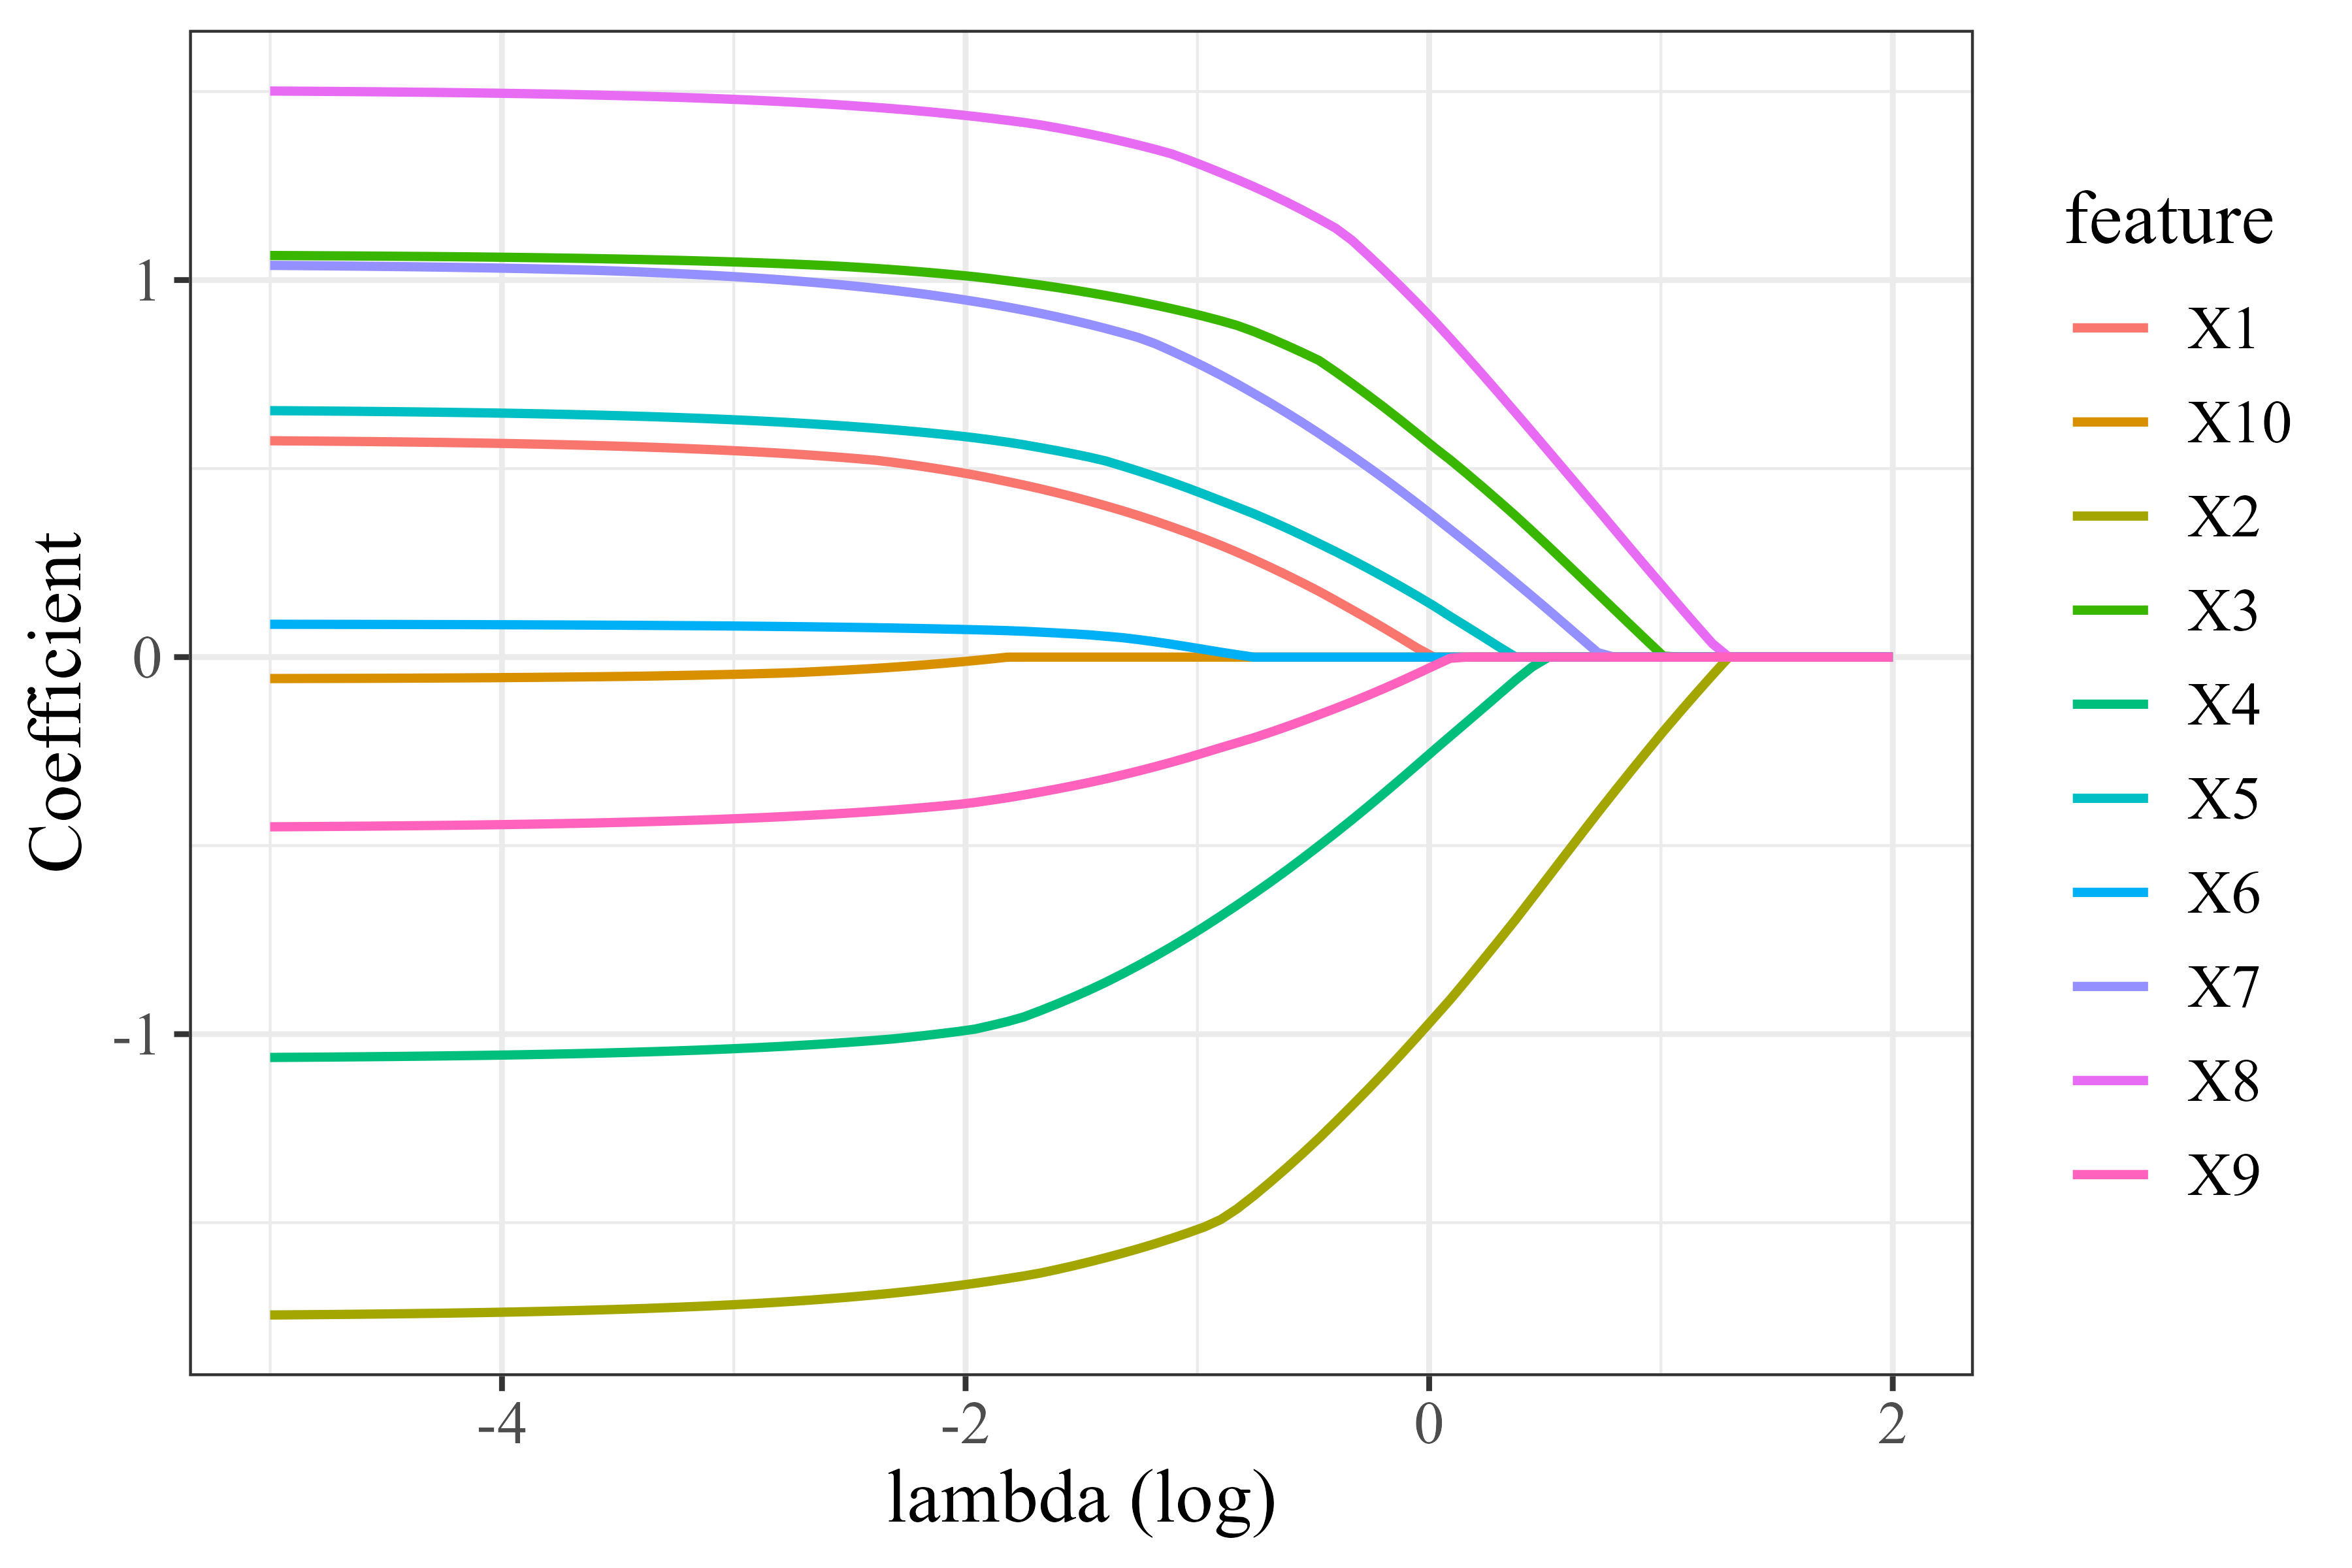
\includegraphics[width=\textwidth]{figs/lambda_path.png}
    \end{subfigure}
    \begin{subfigure}{0.49\textwidth}
        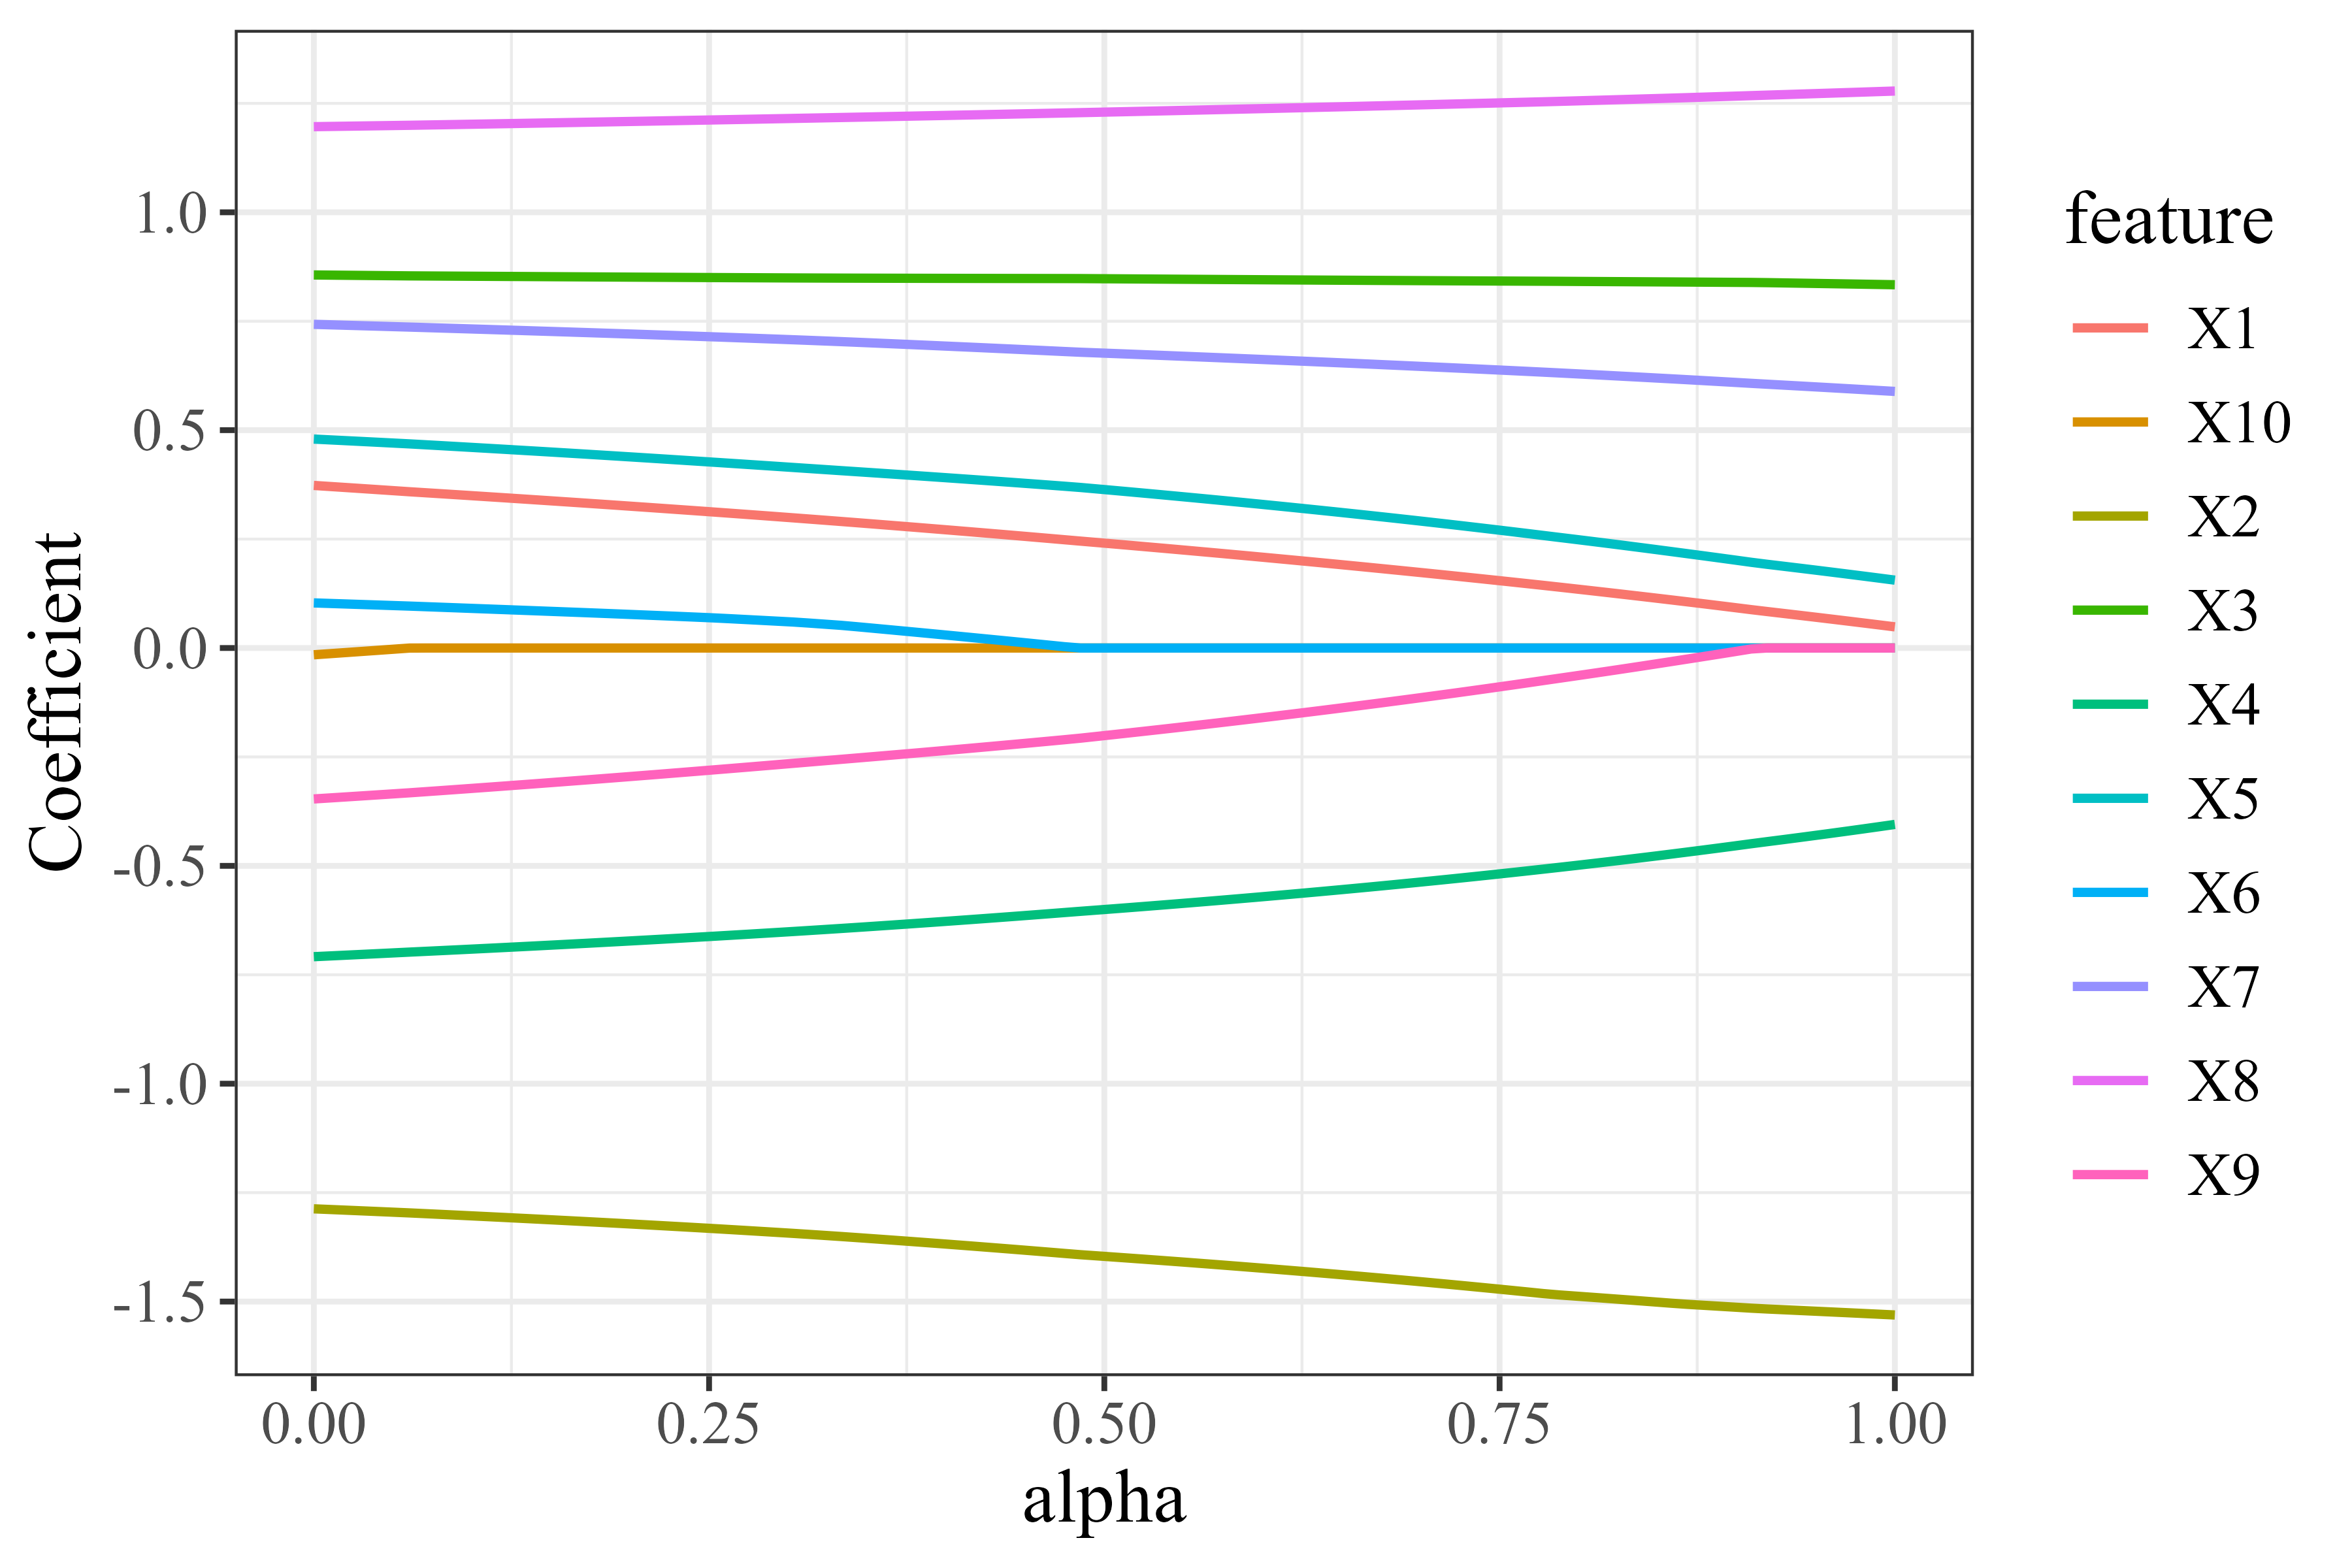
\includegraphics[width=\textwidth]{figs/alpha_path.png}
    \end{subfigure}
    \caption{Coefficient paths of \pkg{capnet} models fitted on the simulated dataset using the \code{coef\_path} function. The left panel plots estimated coefficients as a function of the elastic net penalty parameter $\lambda$. The right panel plots coefficients as a function of the elastic net mixing parameter $\alpha$. These plots illustrate how coefficient shrinkage and sparsity patterns evolve under elastic net regularization in the presence of contribution caps.}
    \label{fig:paths}
\end{figure}

The \code{walk_capnet()} function offers the ability to apply the \code{capnet()} function iteratively over observations in the evaluation set. This is useful because fitting a \pkg{capnet} model over multiple observations can produce an over-penalized model that perform worse in out-of-sample prediction tasks. The walk-forward refitting framework is also useful for time-series tasks, where data arrive sequentially. The \code{walk_capnet()} functions allows for easy sequential fitting and evaluation along the evaluation path. The interface of \code{walk_capnet()} is very similar to that of \code{capnet}, with the exception that it also takes the evaluation dataset \code{newx} as a required input and has an additional optional argument \code{walk}, which controls the step size of the iterative fitting procedure. 

\begin{Code}
    R> fit_walk <- walk_capnet(X, y, L, newx, walk = 1, alpha = alpha, 
    +    lambda = lambda, gamma = gamma)
\end{Code}

\code{walk_capnet()} also returns an \code{S3} object and has accompany \code{coef()} and \code{predict()} methods to display the sequence of coefficients and predictions with the evaluation set.

\begin{CodeChunk}
\begin{CodeInput}
    R> head(coef(walk_fit))
\end{CodeInput}
\begin{CodeOutput}
            intercept        X1        X2        X3         X4        X5
    [1,] -0.010473888 0.5295727 -1.909948 1.2157910 -1.0642892 0.5980203
    [2,] -0.010469909 0.5295734 -1.909942 1.2157780 -1.0642884 0.5980221
    [3,] -0.010472161 0.5295688 -1.909946 1.2157802 -1.0642919 0.5980236
    [4,]  0.017093792 0.4952672 -1.668442 1.0588963 -0.9992213 0.6257662
    [5,] -0.003749633 0.4827738 -1.869136 0.9111731 -1.0221476 0.6174209
    [6,] -0.010472971 0.5295687 -1.909944 1.2157801 -1.0642940 0.5980240
                 X6       X7       X8         X9         X10
    [1,] 0.05092109 1.020880 1.754921 -0.3613088 -0.05495997
    [2,] 0.05093191 1.020894 1.754934 -0.3613085 -0.05495241
    [3,] 0.05093173 1.020889 1.754937 -0.3613081 -0.05495411
    [4,] 0.07342490 1.014856 1.792987 -0.3904655 -0.03321733
    [5,] 0.07924715 1.026394 1.780540 -0.3863961 -0.02650655
    [6,] 0.05093242 1.020889 1.754933 -0.3613079 -0.05495323
\end{CodeOutput}
\end{CodeChunk}

\begin{CodeChunk}
\begin{CodeInput}
    R> tail(predict(walk_fit))
\end{CodeInput}
\begin{CodeOutput}
           prediction
    [15,] -0.73100631
    [16,] -3.24891204
    [17,]  3.03570126
    [18,] -2.56909793
    [19,]  4.42905610
    [20,] -0.05548754
\end{CodeOutput}
\end{CodeChunk}

The \code{cv_capnet()} function implements grid-search cross-validation and has a similar signature to \code{capnet()}. It allows the user to choose the split method (the default is K-fold cross validation) and the loss metrics for measuring prediction or classification accuracy on the held-out sets.\footnote{Currently available metrics include mean-squared error (MSE), out of sample R square, logarithmic loss, brier score, and deviance.} \code{cv_capnet()} allows the user to search for the optimal $\lambda$ and $\alpha$ values individually or simultaneously.

\begin{figure}[h]
    \centering
    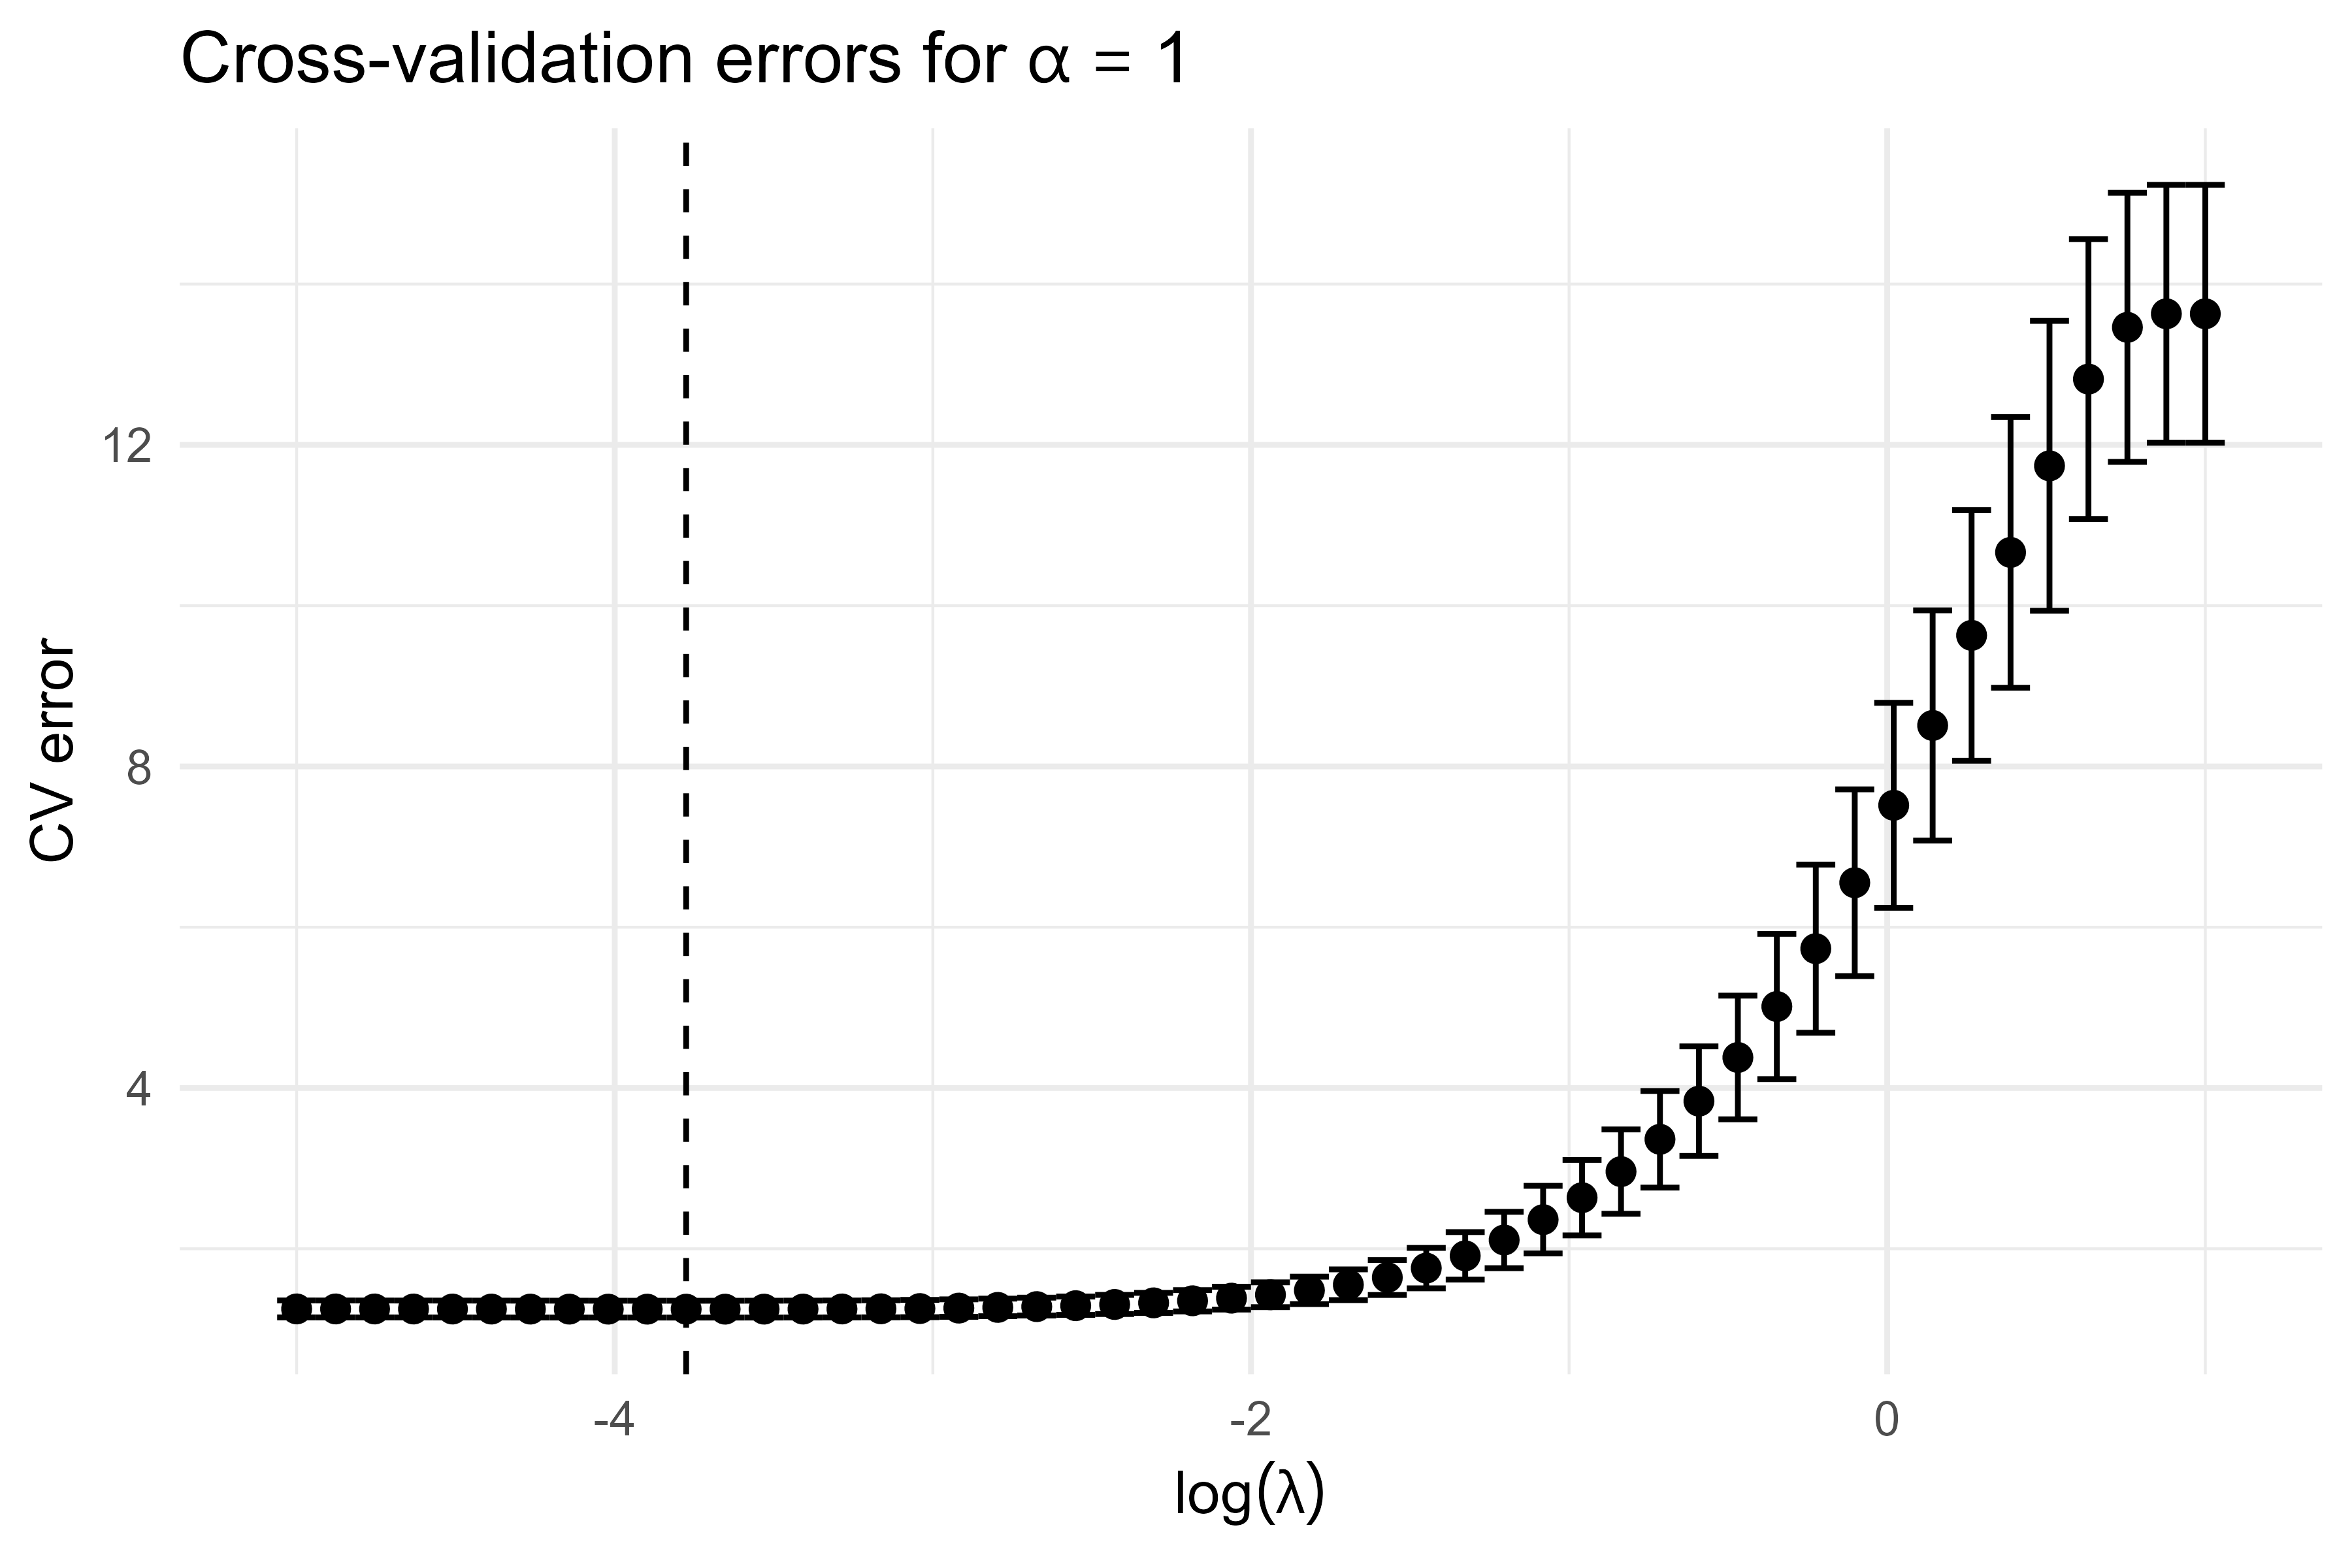
\includegraphics[width=0.75\linewidth]{figs/lambda_cv.png}
    \caption{Cross-validation mean-squared error (MSE) of the \pkg{capnet} model evaluated over a sequence of $\lambda$ values on the simulated dataset. Points represent average validation error across folds, and vertical bars denote variability across folds. The dashed vertical line indicates the selected $\lambda$ minimizing cross-validation error ($\log(\lambda)\approx-3.8$), illustrating the standard model selection procedure implemented in \code{cv\_capnet}.}
    \label{fig:cv_lambda}
\end{figure}

\begin{Code}
    R> gamma <- 0.05
    
    # K-fold grid-search cross-validate on lambda and alpha
    R> cv_fit1 <- cv_capnet(X, y, gamma, L, K = 5)

    # User-specified cross-validation splits
    R> split_id <- rep(1:5, each = 20)
    R> cv_fit2 <- cv_capnet(X, y, gamma, L, splits = split_id)

    # Grid-search on lambda values only
    R> cv_fit3 <- cv_capnet(X, y, gamma, L, 
    +    lambda = exp(seq(1, -5, length.out = 50)), alpha = 0.5)
\end{Code}

Similar to the implementation by \code{cv.glmnet()}, \code{cv_capnet()} uses warm start when searching for \code{lambda} values to cut computational costs. The \code{S3} \code{plot()} method displays the cross-validation curve with upper and lower confidence bounds for each $\lambda$ or $\alpha$ value in the regularization path. Example plots using the simulated data are presented in Figure~\ref{fig:cv_lambda}.

\begin{Code}
    plot(cv_fit1, alpha = 1)
\end{Code}

The package also provides diagnostic tools for examining fitted \pkg{capnet} models. The function \code{capnet\_violations()} identifies where realized feature contributions exceed the specified contribution caps. Given a fitted \pkg{capnet} model, it computes the excess contribution for each feature over the evaluation data. If no new evaluation matrix is supplied, the function uses the same evaluation data that were used when fitting the model. The output includes the row and column indices of all cap violations together with the matrix of excess contributions. The corresponding \code{print()} method displays this excess matrix in sparse form.

\begin{CodeChunk}
\begin{CodeInput}
    R> fit <- capnet(X, y, L, alpha = alpha, lambda = lambda, gamma = 0)
    
    # Default uses the valuation set of the original fit
    R> violations1 <- capnet_violations(fit)

    # User can specify a new valuation set
    R> violations2 <- capnet_violations(fit, newx = tail(newx))
    R> print(violations2)
\end{CodeInput}
\begin{CodeOutput}
               X1 X2     X3     X4 X5 X6     X7     X8 X9      X10
    [15,]       .  . 0.2357      .  .  .      .      .  .        .
    [16,] 0.01699  .      .      .  .  .      .      .  .        .
    [17,]       .  .      .      .  .  .      .      .  . 0.008612
    [18,]       .  .      .      .  .  . 0.3704      .  .        .
    [19,]       .  .      .      .  .  .      . 0.8492  .        .
    [20,]       .  .      . 0.1989  .  .      . 1.5164  .        .
\end{CodeOutput}
\end{CodeChunk}

The function \code{plot\_redistribution()} compares two fitted \pkg{capnet} models in terms of both their coefficients and their average feature contributions over the evaluation data. It supports two display modes: side-by-side bar charts showing the raw values for each model, and difference plots showing how coefficients and contributions change from one model to the other. Figure~\ref{fig:redistribute} shows a side-by-side comparison between an uncapped and a capped model fitted on the simulated dataset.

\begin{figure}[h]
    \centering
    \begin{subfigure}{0.49\textwidth}
        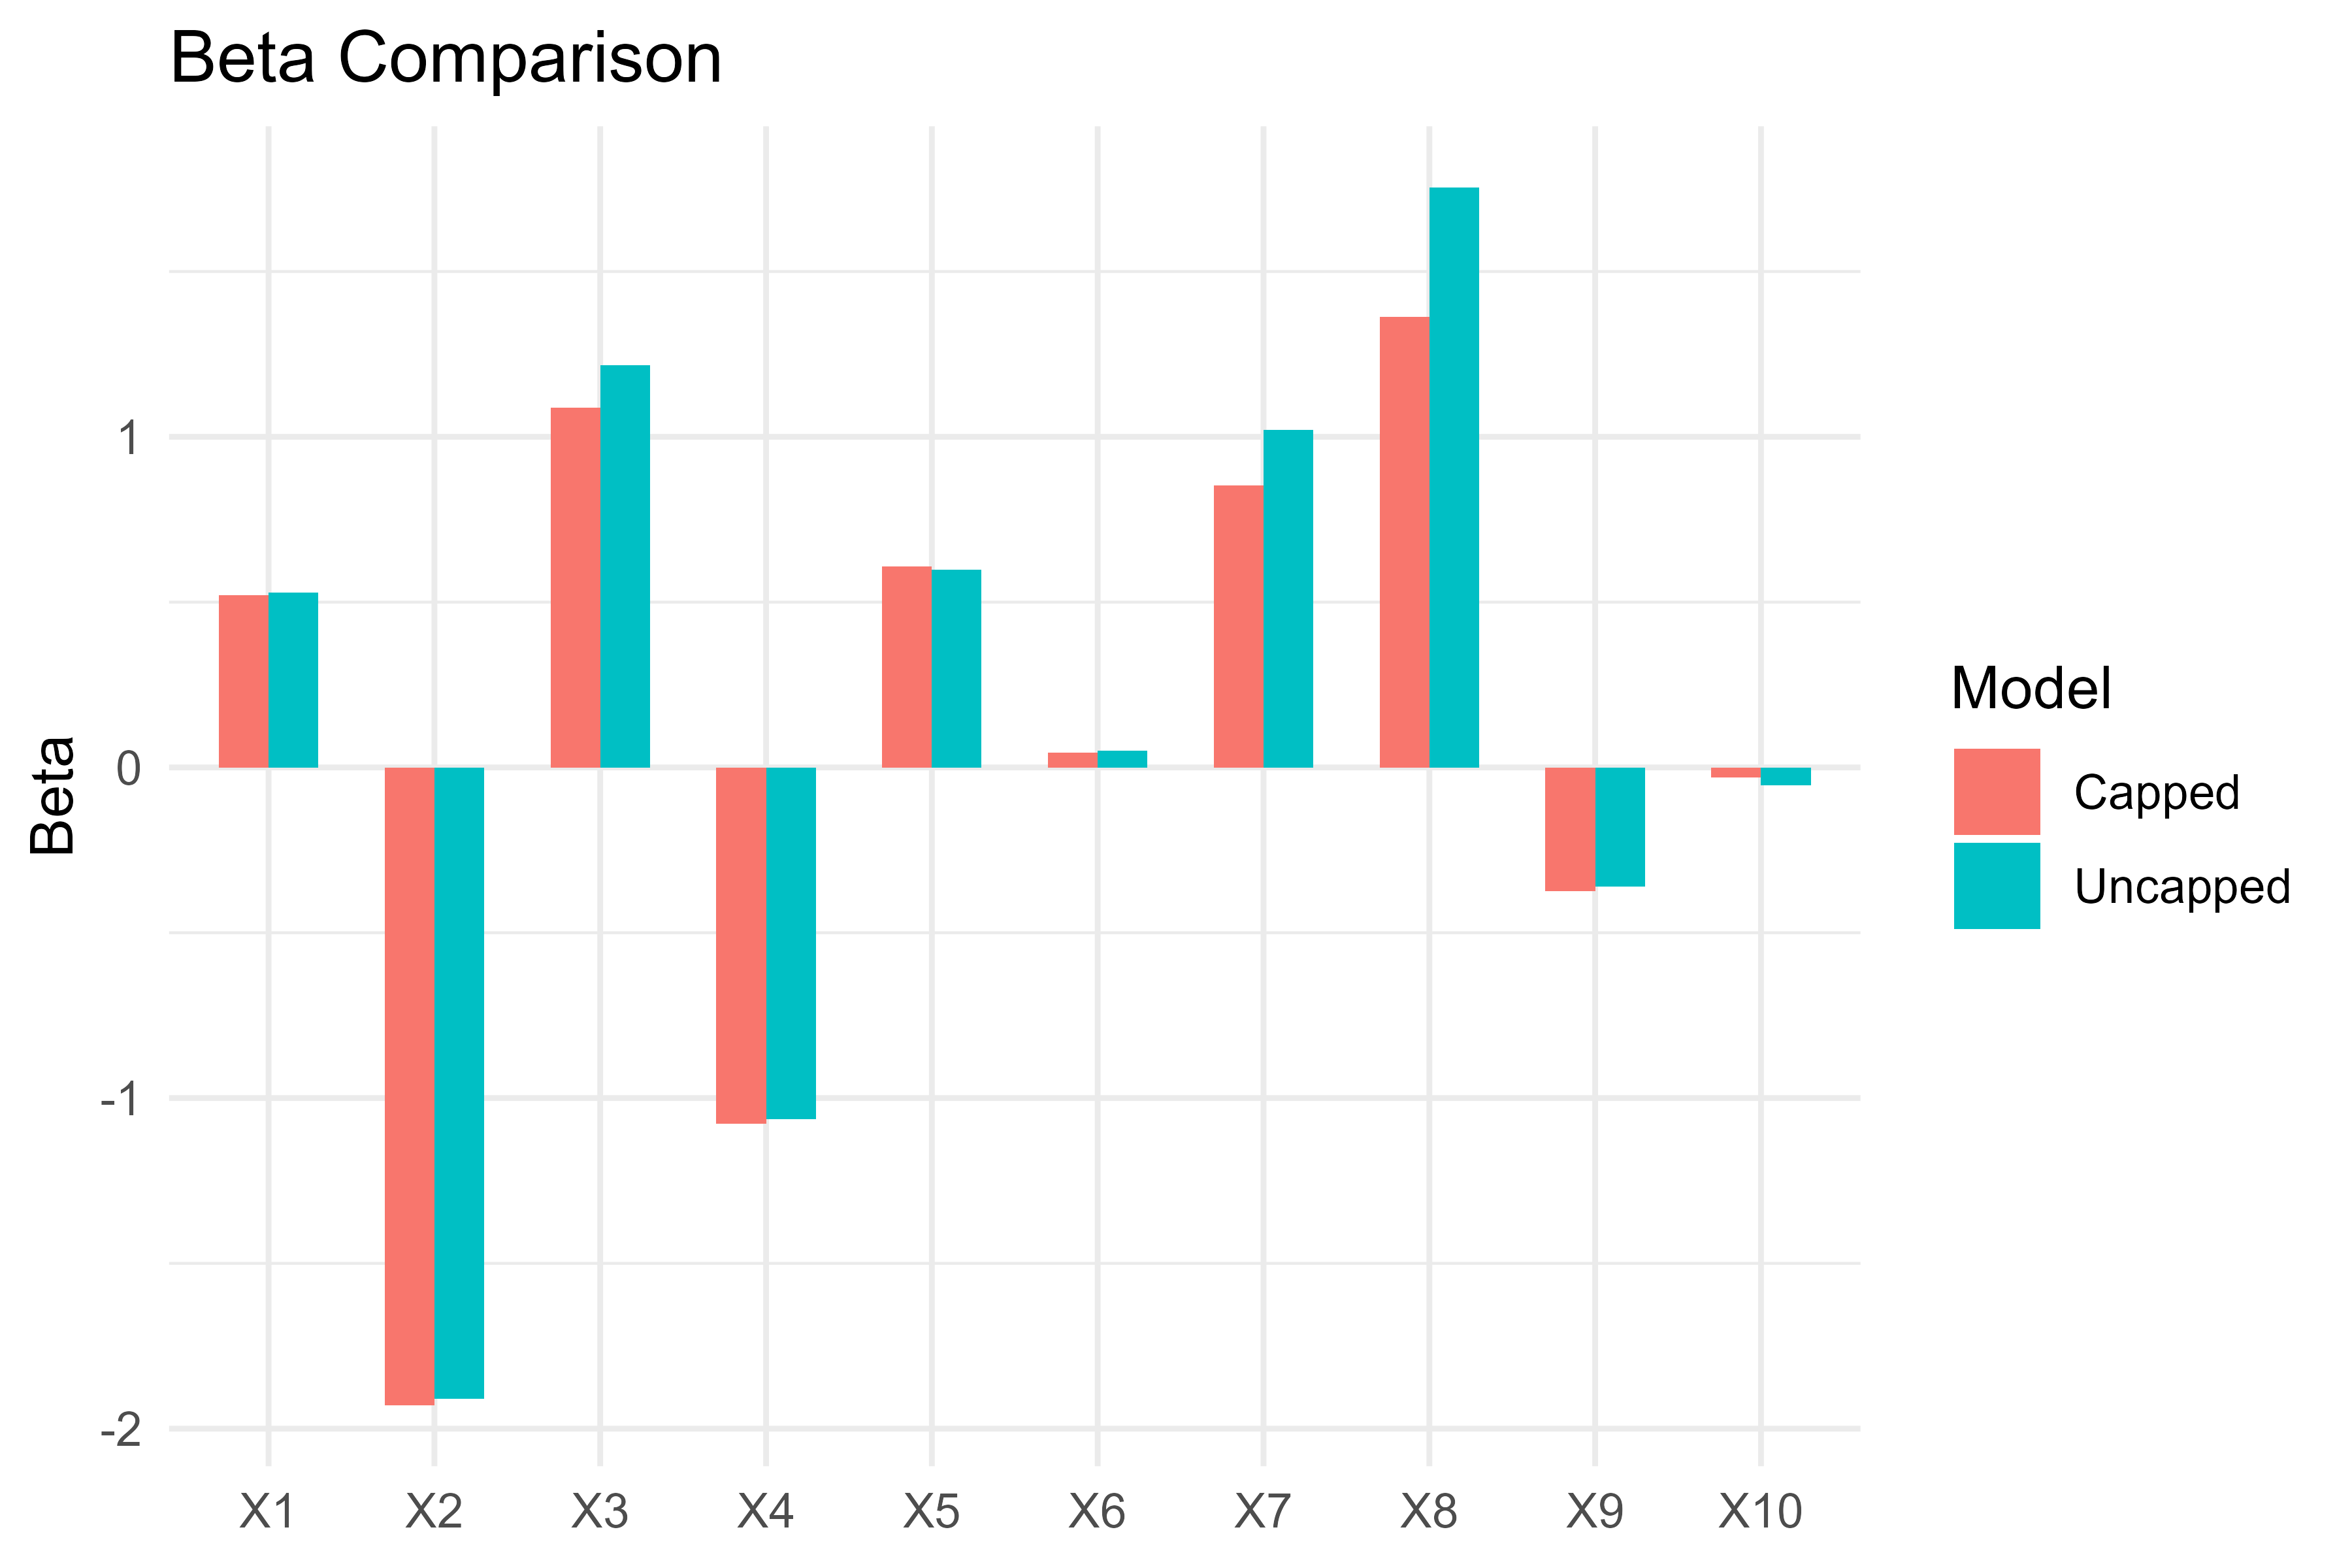
\includegraphics[width=\textwidth]{figs/beta_redistribute.png}
    \end{subfigure}
    \begin{subfigure}{0.49\textwidth}
        
\includegraphics[width=\textwidth]{figs/contrib_redistribute.png}
    \end{subfigure}
    \caption{Comparison of coefficient values (left panel) and average feature contributions (right panel) between capped and uncapped \pkg{capnet} models fitted on the simulated dataset. Results are generated using \code{plot\_redistribution()} applied to two fitted models with different contribution penalties. Imposing contribution caps reduces the magnitude of coefficients associated with high-impact features (e.g. $X3$, $X7$, $X8$) and redistributes predictive weight to other predictors, demonstrating how \pkg{capnet} enforces balanced feature influence.}
    \label{fig:redistribute}
\end{figure}

\begin{Code}
    R> newx <- newx[1:5,]
    R> fit1 <- capnet(X, y, L, alpha = alpha, lambda = lambda, gamma = 0)
    R> fit2 <- capnet(X, y, L, alpha = alpha, lambda = lambda, gamma = 10)

    # Side-by-side bar chart comparing feature coefficients and contributions
    R> plot_redistribution(fit1, fit2, plot = "delta")

    # Bar chart showing changes in feature coefficients and contributions
    R> plot_redistribution(fit1, fit2, plot = "raw")
\end{Code}


\section{Applications}\label{sec:examples}

An important application of \pkg{capnet} arises in quantitative finance, where predictor variables frequently exhibit heavy-tailed distributions and episodic extremes. In such environments, standard linear models can produce unstable and economically undesirable predictions, as a small number of extreme feature realizations may dominate the model output. From a portfolio construction perspective, this translates into concentrated exposures and fragile positions that are highly sensitive to outliers. Risk managers may be concerned with these dynamics, as they can lead to unintended bets, amplified drawdowns, and poor tail-risk properties. In practice, portfolio managers often impose explicit constraints---such as position limits, exposure caps, or risk budgets---to control the influence of individual signals. These constraints reflect a preference for diversification not only at the portfolio level but also at the level of predictive signals. However, conventional penalized regression methods (e.g., ridge or elastic net) shrink coefficients uniformly and do not directly control the realized contribution of each feature. As a result, even regularized models can produce predictions dominated by a single extreme predictor when its realized value is large. The contribution-based framework implemented in \pkg{capnet} directly addresses this issue by penalizing excessive feature contributions, thereby aligning statistical estimation with practical risk management objectives. The time-series nature of financial data further necessitates rolling estimation procedures, for which the walk-forward implementation \code{walk_capnet} is particularly well suited.

To illustrate the empirical performance of \pkg{capnet}, we use data from the \href{https://www.kaggle.com/competitions/hull-tactical-market-prediction}{Hull Tactical Market Prediction Kaggle competition}. This dataset contains daily observations combining publicly available market data with proprietary features designed to predict excess returns of the S\&P 500. Following the variable selection of the competition’s baseline model, we construct a backtesting pipeline to evaluate alternative approaches to imposing contribution caps within a linear modeling framework.

\begin{table}[ht]
\centering
\begin{tabular}{lccc}
    \hline\hline
    Variable & Mean & Variance & Excess Kurtosis \\ 
    \hline
    S2 & 0.03 & 1.04 & -0.40 \\ 
    E2 & 0.51 & 2.01 & -0.16 \\ 
    E3 & 0.36 & 2.27 & -0.32 \\ 
    P9 & 0.39 & 0.15 & -1.53 \\ 
    S1 & 0.24 & 2.00 & 1.13 \\ 
    S5 & 0.03 & 1.27 & 14.56 \\ 
    I2 & -0.51 & 1.57 & 1.66 \\ 
    P8 & 1.55 & 0.50 & 2.87 \\ 
    P10 & 1.47 & 0.66 & 0.34 \\ 
    P12 & -0.01 & 1.21 & 11.01 \\ 
    P13 & 0.51 & 0.08 & -1.11 \\
    \hline\hline
\end{tabular}
\caption{Summary statistics of selected variables from the Kaggle dataset. Features $S5$ and $P12$ exhibit substantial positive kurtosis.}
\label{tab:variable}
\end{table}

Table~\ref{tab:variable} reports summary statistics for selected variables. While most variables exhibit moderate dispersion, $S5$ and $P12$ display pronounced leptokurtosis. These distributional properties imply that extreme realizations occur more frequently than would be expected under Gaussian assumptions. In a standard linear model, such features can exert disproportionate influence on predictions, particularly when extreme values arise out of sample but are not well represented in the training data. This mismatch between in-sample estimation and out-of-sample realization is a key source of model instability and motivates the use of contribution-based regularization.

We consider three modeling approaches: (i) an uncapped baseline, (ii) a post-fit capping method, and (iii) the walk-forward \pkg{capnet} approach. At each monthly refit date, models are estimated using a 20-year rolling training window and used to generate predictions for the subsequent month. Given training data \code{x_train}, \code{y_train}, test data \code{x_test}, and a specified contribution cap vector \code{L}, we estimate \code{capnet} or \code{walk_capnet} models with \code{alpha = 0.5} and a regularization parameter \code{lambda} selected via \code{cv.glmnet}. For the post-fit capping approach, we first estimate the uncapped model (equivalently, \code{capnet} with \code{gamma = 0}) and then apply contribution caps to the fitted model ex post. While this guarantees that realized contributions satisfy the cap constraint, it does not allow the model to adjust coefficients in response to the constraint during estimation. In contrast, \pkg{capnet} incorporates the cap penalty directly into the objective function, allowing the model to reallocate weight across predictors in a manner that balances predictive accuracy with contribution control. The backtest spans January 1, 2020 through February 13, 2026. For the walk-forward specification, we evaluate multiple values of the penalty parameter \code{gamma} to assess sensitivity to the strength of the cap penalty. Table~\ref{tab:elan_result} reports the average out-of-sample $R^2$ across specifications.

\begin{table}[h]
    \centering
    \begin{tabular}{l|c|c}
    \hline\hline\\[-2.7ex]
        Method & $\gamma$ & OOS $R^2$ \\
        \hline
        Uncapped & & 0.00706 \\
        Post-fit Cap & & 0.00573 \\
        Capnet & 0.1 & 0.00739 \\
        Capnet & 1 & 0.00766 \\
        Capnet & 10 & 0.00758 \\
        Capnet & 100 & 0.00764\\
    \hline\hline
    \end{tabular}
    \caption{Average out-of-sample $R^2$ from the backtest experiment (January 2020 to February 2026) on the Kaggle dataset. The \pkg{capnet} models achieve performance comparable to or exceeding the uncapped model while substantially outperforming the post-fit approach, indicating that incorporating contribution constraints during estimation provides a more effective approach in accounting for feature influence.}
    \label{tab:elan_result}
\end{table}

To provide a more granular comparison over time, Figure~\ref{fig:oosrsq} presents rolling out-of-sample $R^2$ computed over a 252-day window. The uncapped model (blue) exhibits substantial performance volatility, including large negative deviations that correspond to periods where extreme feature realizations dominate predictions. The post-fit capping approach reduces these downside outcomes and improves robustness during periods of broad underperformance, but at the cost of attenuating strong predictive signals when they are present. In contrast, the walk-forward \pkg{capnet} model achieves a more favorable trade-off. By incorporating contribution control during estimation, it selectively dampens the influence of extreme realizations while preserving informative variation in the predictors. This leads to a smoother performance profile with fewer large drawdowns and more consistentout-of-sample $R^2$. From a portfolio perspective, this corresponds to improved stability and more reliable signal extraction over time.

\begin{figure}[h]
    \centering
    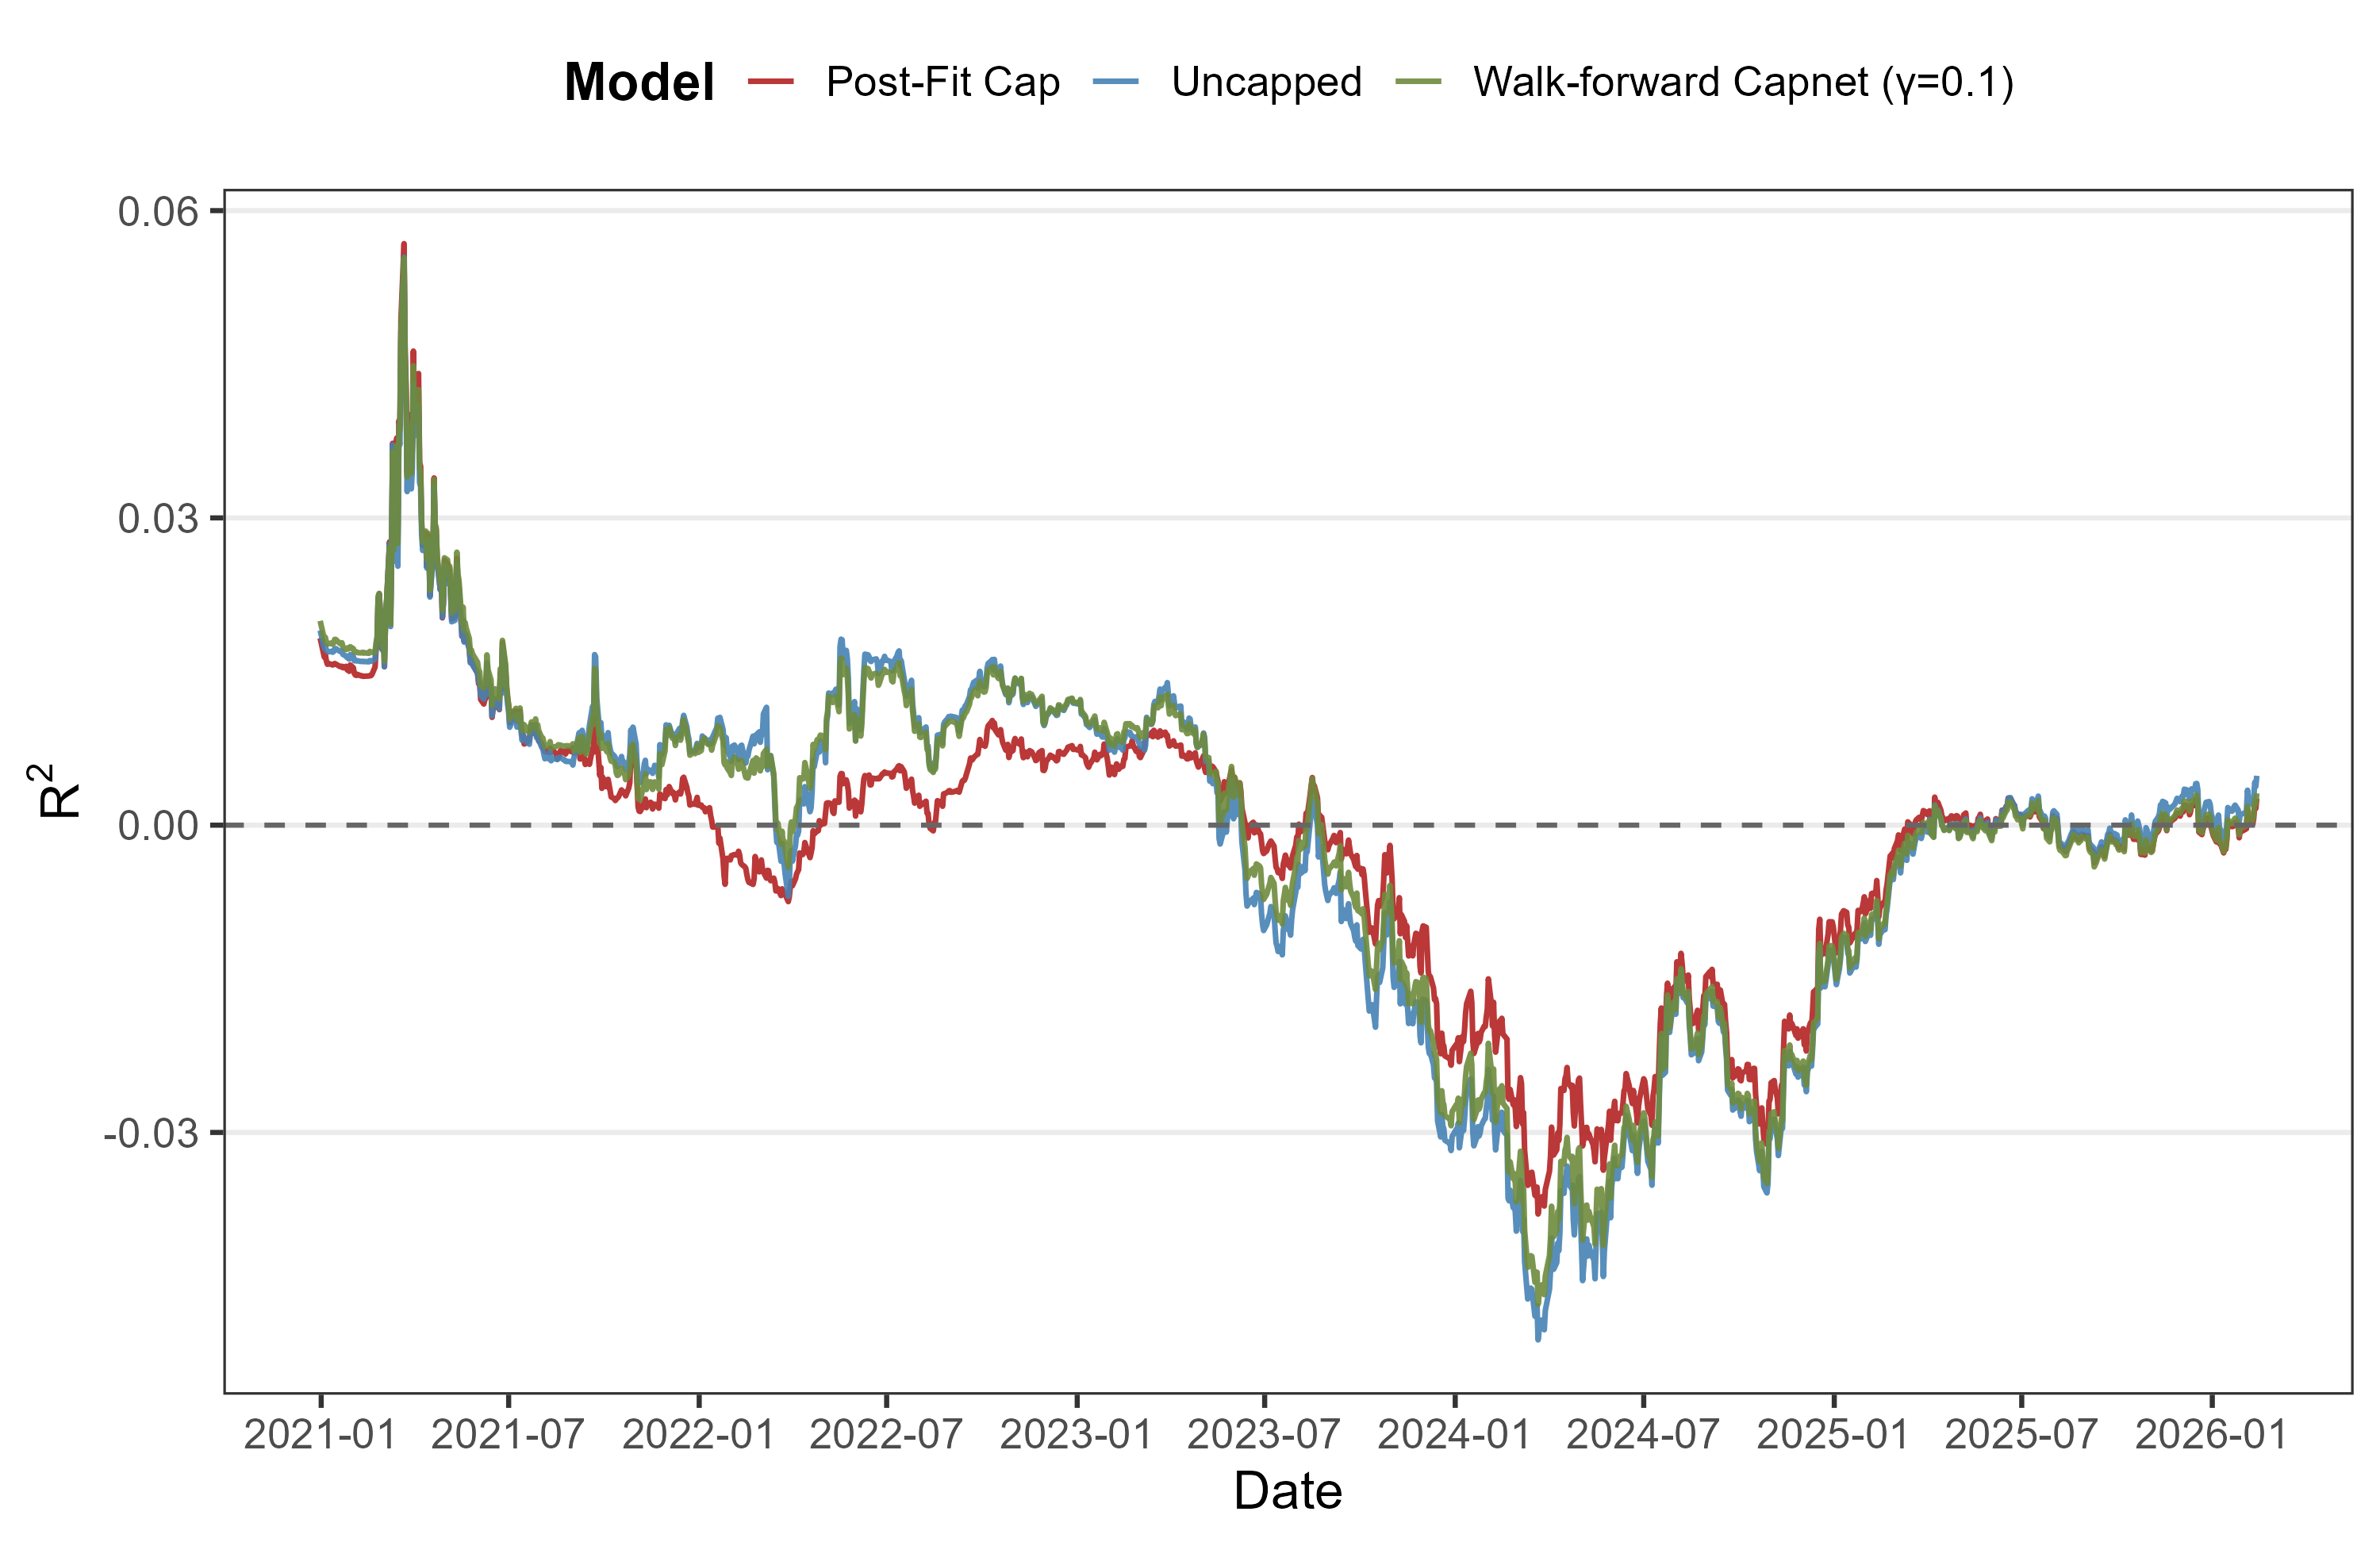
\includegraphics[width=0.75\linewidth]{figs/oosrsq.png}
    \caption{Rolling out-of-sample $R^2$ computed over a 252-day window for three models: uncapped (blue), post-fit capped (red), and walk-forward \pkg{capnet} (green). The uncapped model exhibits substantial performance volatility, including large negative deviations certain periods. The post-fit approach achieves more stable predictive power but attenuates strong signals. The walk-forward \pkg{capnet} model achieves a smoother and more stable performance profile.}
    \label{fig:oosrsq}
\end{figure}

The performance gains observed for \pkg{capnet} can be traced to its ability to regulate feature-level contributions rather than merely shrinking coefficients. In the uncapped model, a small number of predictors have concentrated contributions, resulting in unstable predictions and large drawdowns in performance. Post-fit capping mitigates this effect by truncating contributions ex post, but does not allow the model to adjust its coefficients accordingly. In contrast, \pkg{capnet} incorporates contribution constraints directly into the estimation problem, enabling the model to redistribute predictive weight across features. This leads to a more balanced contribution structure and improved stability over time.

\begin{figure}[h]
    \centering
    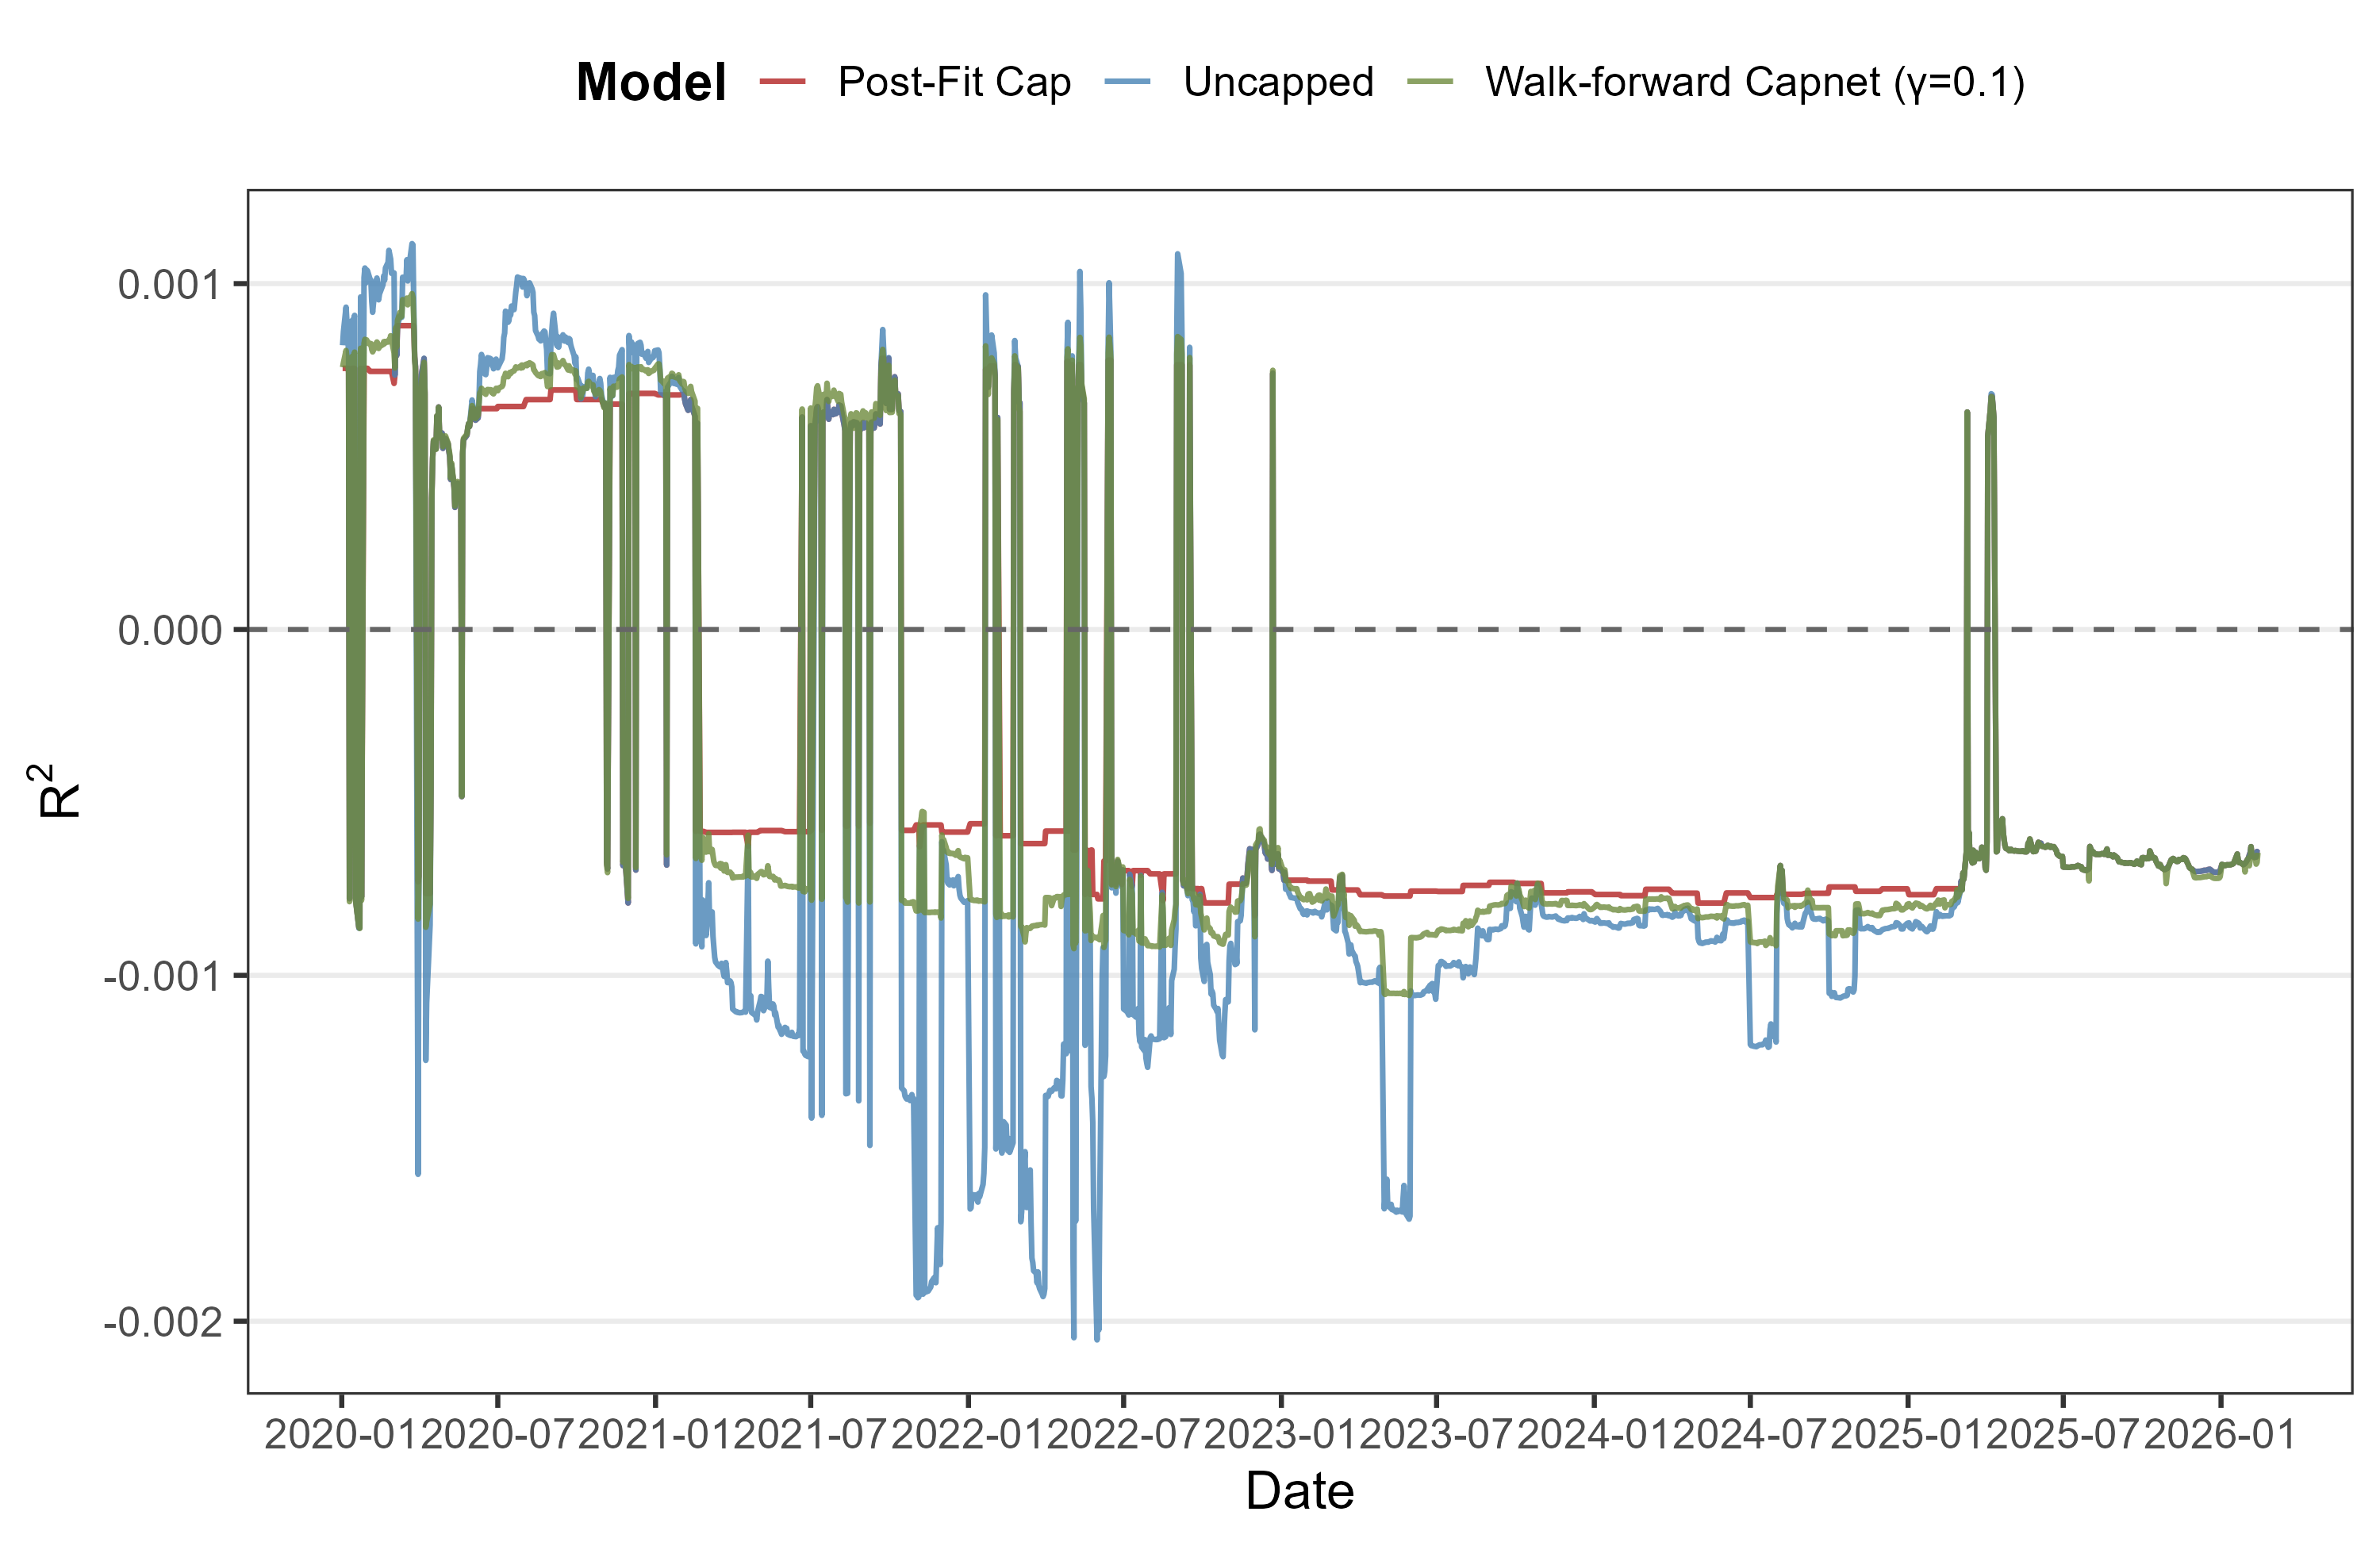
\includegraphics[width=0.75\linewidth]{figs/max_contributions.png}
    \caption{Time series of the maximum absolute feature contribution at each out-of-sample prediction for the uncapped (blue), post-fit capped (red), and walk-forward \pkg{capnet} (green) models. The post-fit approach enforces a hard cap, truncating contributions at the specified limit. In contrast, \pkg{capnet} imposes a soft constraint via the penalty parameter $\gamma$, reducing extreme contributions while preserving flexibility when large contributions are informative.}
    \label{fig:max_contrib}
\end{figure}

Figure~\ref{fig:max_contrib} plots the contribution of the feature with the largest absolute contribution at each prediction point. By construction, the post-fit capping approach enforces a hard constraint, keeping contributions at or within the cap boundary $L$. In contrast, \pkg{capnet} imposes a soft constraint through the penalty parameter $\gamma$. For example, with $\gamma = 0.1$, contributions are moderated relative to the uncapped model but are not mechanically truncated at the cap. This allows the model to retain flexibility when extreme contributions are informative, while still discouraging excessive concentration.

To further illustrate how \pkg{capnet} redistributes feature contributions, Table~\ref{tab:contributions} reports a snapshot for May 24, 2023. In the uncapped model, features E2 and P8 violate the contribution caps. The post-fit capping approach enforces the constraint mechanically, reducing these contributions without adjusting other coefficients. In contrast, the walk-forward \pkg{capnet} model modifies multiple coefficients simultaneously, redistributing contributions across features. This reflects the model’s ability to internalize the constraint and solve a constrained optimization problem rather than applying an ex post correction.

\begin{table}[h]
    \centering
    \begin{tabular}{lccc}
    \hline\hline
        Feature & Uncapped & Post-Fit Cap & Walk-forward \pkg{capnet} \\
    \hline
        S2 & $-3.439$ & $-3.439$ & $-3.380$ \\
        E2 & $-0.140$ & $-0.112$ & $-0.637$ \\
        E3 & $0$ & $0$ & $0$ \\
        P9 & $0.124$ & $0.124$ & $0.075$ \\
        S1 & $-0.156$ & $-0.156$ & $-0.005$ \\
        S5 & $0.073$ & $0.073$ & $0.073$ \\
        I2 & $-4.863$ & $-4.863$ & $-5.357$ \\
        P8 & $-16.07$ & $-7.707$ & $-10.47$ \\
        P10 & $0$ & $0$ & $-0.298$ \\
        P12 & $0.743$ & $0.743$ & $0.883$ \\
        P13 & $-0.641$ & $-0.641$ & $-0.495$ \\
    \hline\hline
    \end{tabular}
    \caption{Feature-level contributions for the uncapped, post-fit capped, and walk-forward \pkg{capnet} models on May 24, 2023. All values are scaled by $10^4$ for readability. In the uncapped model, features such as $E2$ and $P8$ exceed the contribution ceilings. The post-fit method enforces cap mechanically without adjusting other coefficients. In contrast, the \pkg{capnet} model redistributes contributions across multiple features.}
    \label{tab:contributions}
\end{table}

From a computational perspective, \code{capnet} achieves runtime comparable to \code{glmnet} under the same specification. Table~\ref{tab:runtime} reports the total runtime of the monthly refit backtesting procedure for three methods. All experiments were performed on a machine with an Intel i7-7700 CPU (4 cores, 3.6 GHz) and 32 GB RAM. At each refit date, both the \code{glmnet} and \code{capnet} approaches perform a single cross-validation search to select $\lambda$, followed by one model fit using the full training sample. In contrast, the \code{walk\_capnet} approach also performs a cross-validation step at each refit date but subsequently refits the model sequentially for each out-of-sample observation. This repeated fitting leads to a higher overall computational cost.

\begin{table}[h]
    \centering
    \begin{tabular}{lc}
    \hline\hline
        Model & Runtime (secs) \\
    \hline
        \code{glmnet} & 13.06 \\
        \code{capnet} & 16.05 \\
        \code{walk_capnet} & 58.87 \\
    \hline\hline
    \end{tabular}
    \caption{Total runtime (in seconds) of the monthly refit backtesting procedure for each method. Both \code{glmnet} and \code{capnet} perform a single cross-validation step and model fit at each refit date, while \code{walk\_capnet} additionally refits the model sequentially for each out-of-sample observation, resulting in higher computational cost.}
    \label{tab:runtime}
\end{table}

\section{Conclusion}\label{sec:conclusion}

This paper introduced \pkg{capnet}, an \proglang{R} package for fitting generalized linear models with contribution-capped regularization. The proposed framework extends classical penalized regression methods by directly constraining the realized contributions of predictors to the linear predictor. By shifting the focus of regularization from coefficients to feature-level influence, \pkg{capnet} addresses a class of modeling problems in which extreme covariate realizations can disproportionately affect predictions.

The contribution-cap formulation integrates naturally with generalized linear models and yields a convex optimization problem that can be efficiently solved using limited-memory quasi-Newton methods. The ability to specify an evaluation matrix distinct from the training data further enhances flexibility, allowing users to enforce stability not only in-sample but also in stress scenarios or anticipated deployment environments. The package provides a practical implementation of this framework, including tools for model fitting, cross-validation, sequential estimation, and diagnostic analysis, with an interface designed to be consistent with established workflows.

Empirical results demonstrate that contribution-based regularization can improve predictive stability and performance in settings with heavy-tailed predictors. In particular, \pkg{capnet} reduces the dominance of individual predictors by redistributing predictive weight across features, leading to smoother out-of-sample performance and fewer extreme deviations. Compared to post-hoc capping approaches, which enforce constraints after estimation, \pkg{capnet} incorporates these constraints directly into the optimization problem, resulting in a more coherent and effective trade-off between robustness and predictive accuracy.

Several limitations and directions for future research remain. The selection of contribution caps requires domain knowledge or heuristic procedures, and developing principled, data-driven approaches for tuning these parameters is an important area for further work. In addition, while the current implementation scales well to moderate evaluation sets, extending the framework to very large or streaming evaluation matrices may require additional computational strategies. Finally, further exploration of the relationship between contribution-based regularization and other robustness frameworks, such as distributionally robust optimization, may yield useful theoretical and practical insights.

Overall, \pkg{capnet} expands the toolkit of penalized regression by introducing a new dimension of control over model behavior. By aligning statistical estimation with practical constraints on predictor influence, it provides a flexible and interpretable framework for applications in which stability, robustness, and feature-level interpretability are of central importance.

\newpage
\bibliography{refs}

\end{document}
